% Font options: 10pm, 11pt, 12pt
% Align headings left instead of center: nocenter
\documentclass[xcolor=x11names,compress]{beamer}\usepackage[]{graphicx}\usepackage[]{color}
%% maxwidth is the original width if it is less than linewidth
%% otherwise use linewidth (to make sure the graphics do not exceed the margin)
\makeatletter
\def\maxwidth{ %
  \ifdim\Gin@nat@width>\linewidth
    \linewidth
  \else
    \Gin@nat@width
  \fi
}
\makeatother

\definecolor{fgcolor}{rgb}{0.345, 0.345, 0.345}
\newcommand{\hlnum}[1]{\textcolor[rgb]{0.686,0.059,0.569}{#1}}%
\newcommand{\hlstr}[1]{\textcolor[rgb]{0.192,0.494,0.8}{#1}}%
\newcommand{\hlcom}[1]{\textcolor[rgb]{0.678,0.584,0.686}{\textit{#1}}}%
\newcommand{\hlopt}[1]{\textcolor[rgb]{0,0,0}{#1}}%
\newcommand{\hlstd}[1]{\textcolor[rgb]{0.345,0.345,0.345}{#1}}%
\newcommand{\hlkwa}[1]{\textcolor[rgb]{0.161,0.373,0.58}{\textbf{#1}}}%
\newcommand{\hlkwb}[1]{\textcolor[rgb]{0.69,0.353,0.396}{#1}}%
\newcommand{\hlkwc}[1]{\textcolor[rgb]{0.333,0.667,0.333}{#1}}%
\newcommand{\hlkwd}[1]{\textcolor[rgb]{0.737,0.353,0.396}{\textbf{#1}}}%
\let\hlipl\hlkwb

\usepackage{framed}
\makeatletter
\newenvironment{kframe}{%
 \def\at@end@of@kframe{}%
 \ifinner\ifhmode%
  \def\at@end@of@kframe{\end{minipage}}%
  \begin{minipage}{\columnwidth}%
 \fi\fi%
 \def\FrameCommand##1{\hskip\@totalleftmargin \hskip-\fboxsep
 \colorbox{shadecolor}{##1}\hskip-\fboxsep
     % There is no \\@totalrightmargin, so:
     \hskip-\linewidth \hskip-\@totalleftmargin \hskip\columnwidth}%
 \MakeFramed {\advance\hsize-\width
   \@totalleftmargin\z@ \linewidth\hsize
   \@setminipage}}%
 {\par\unskip\endMakeFramed%
 \at@end@of@kframe}
\makeatother

\definecolor{shadecolor}{rgb}{.97, .97, .97}
\definecolor{messagecolor}{rgb}{0, 0, 0}
\definecolor{warningcolor}{rgb}{1, 0, 1}
\definecolor{errorcolor}{rgb}{1, 0, 0}
\newenvironment{knitrout}{}{} % an empty environment to be redefined in TeX

\usepackage{alltt}
%\documentclass[xcolor=x11names,compress,handout]{beamer}
\usepackage[]{graphicx}
\usepackage[]{color}
\usepackage{booktabs}
\usepackage{hyperref}
\usepackage{tikz}
\usepackage{multirow}
\usepackage{dcolumn}
\usepackage{bigstrut}
\usepackage{amsmath} 
\usepackage{xcolor,colortbl}
\usepackage{amssymb}
%\newcommand{\done}{\cellcolor{teal}#1}

%% Beamer Layout %%%%%%%%%%%%%%%%%%%%%%%%%%%%%%%%%%
\useoutertheme[subsection=false,shadow]{miniframes}
\useinnertheme{default}
\usefonttheme{serif}
\usepackage{Arev}
\usepackage{pdfpages}

\setbeamerfont{title like}{shape=\scshape}
\setbeamerfont{frametitle}{shape=\scshape, size=\normalsize}

\definecolor{dkblue}{RGB}{0,0,102}

\setbeamercolor*{lower separation line head}{bg=dkblue} 
\setbeamercolor*{normal text}{fg=black,bg=white} 
\setbeamercolor*{alerted text}{fg=red} 
\setbeamercolor*{example text}{fg=black} 
\setbeamercolor*{structure}{fg=black} 
 
\setbeamercolor*{palette tertiary}{fg=black,bg=black!10} 
\setbeamercolor*{palette quaternary}{fg=black,bg=black!10} 

\renewcommand{\(}{\begin{columns}}
\renewcommand{\)}{\end{columns}}
\newcommand{\<}[1]{\begin{column}{#1}}
\renewcommand{\>}{\end{column}}

\setbeamertemplate{navigation symbols}{} 
\setbeamertemplate{footline}[frame number]
\setbeamertemplate{caption}{\raggedright\insertcaption\par}

\setbeamersize{text margin left=5pt,text margin right=5pt}

%%%%%%%%%%%%%%%%%%%%%%%%%%%%%%%%%%%%%%%%%%%%%%%%%%


\title{Making Causal Critiques}
\subtitle{Day 2 - Fundamental Critiques}
\author{Jonathan Phillips}
\IfFileExists{upquote.sty}{\usepackage{upquote}}{}
\begin{document}

\frame{\titlepage}

\section{Introduction}

\begin{frame}
\frametitle{What do political scientists \textbf{know}?}
\begin{itemize}
\item Door-to-door political campaigning works
\item Proportional Representation electoral systems have more parties
\item Democracies do not go to war with each other
\item Development helps democracies endure
\item ...And that's about it
\end{itemize}
\end{frame}

\begin{frame}
\frametitle{What do political scientists \textbf{know}?}
\begin{itemize}
\item Thousands of books and papers have \textit{not} generated any causal knowledge
\begin{itemize}
\item Many add \textbf{descriptive} knowledge
\item Many investigate \textbf{specific} events, not generalizable variables
\item Many highlight \textbf{correlations} between variables
\end{itemize}
\end{itemize}
\end{frame}

\begin{frame}
\frametitle{What do political scientists \textbf{know}?}
\begin{itemize}
\item \textbf{Correlation is not causation}
\begin{itemize}
\item If we look hard enough we can always find correlations
\item By chance...
\item Due to complex social patterns...
\item But we cannot conclude that there is a causal effect of $x$ on $y$
\end{itemize}
\item \textit{More} data will not help
\item The problem is the \textit{type} of data; it does not allow us to answer causal question 
\end{itemize}
\end{frame}

\setbeamercolor{background canvas}{bg=}
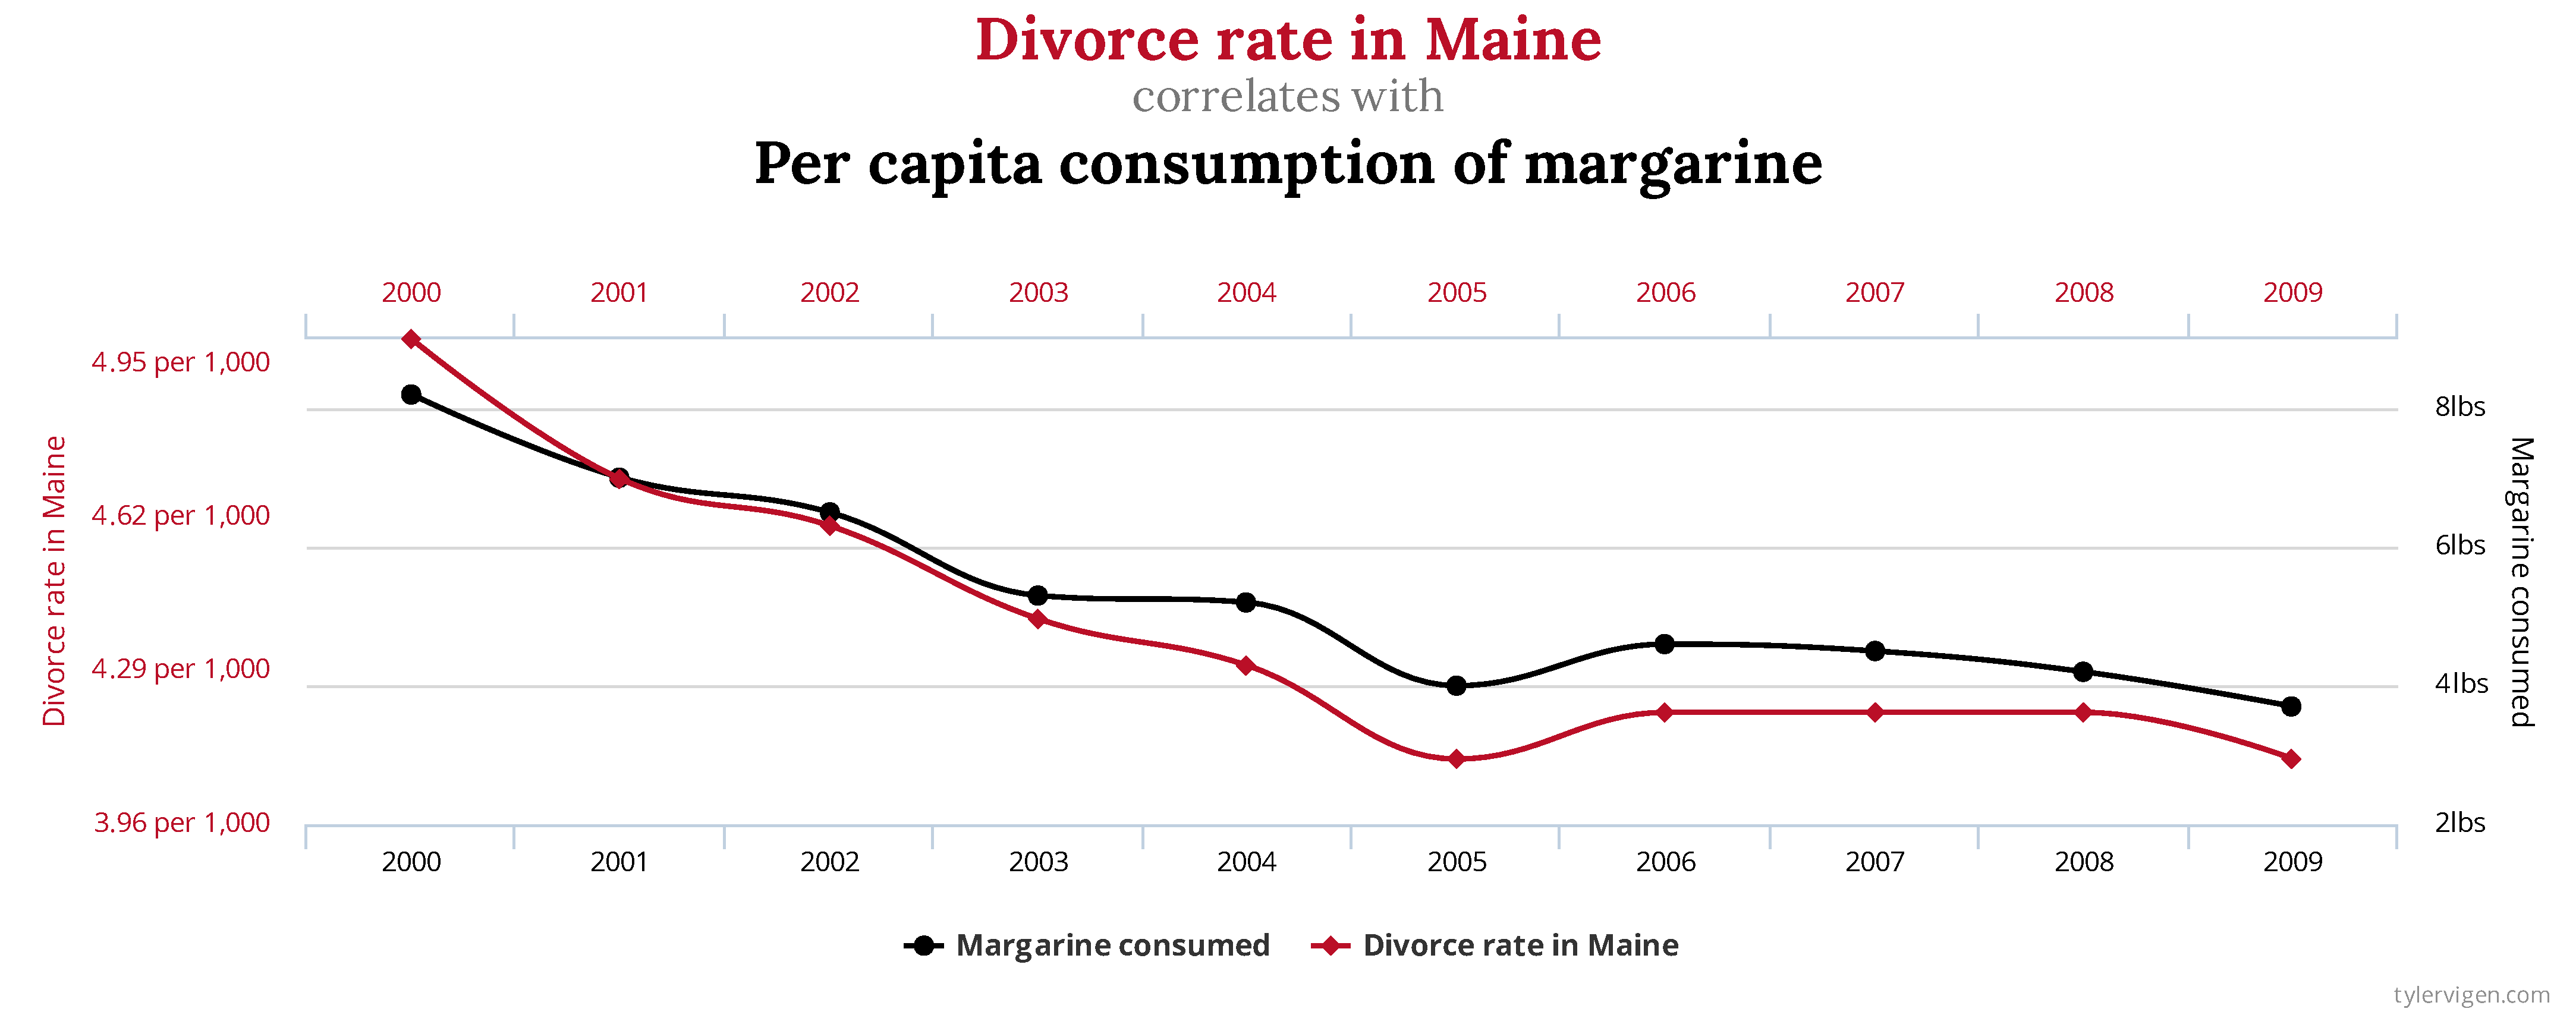
\includepdf[pages={1}]{chart_1.pdf}

\setbeamercolor{background canvas}{bg=}
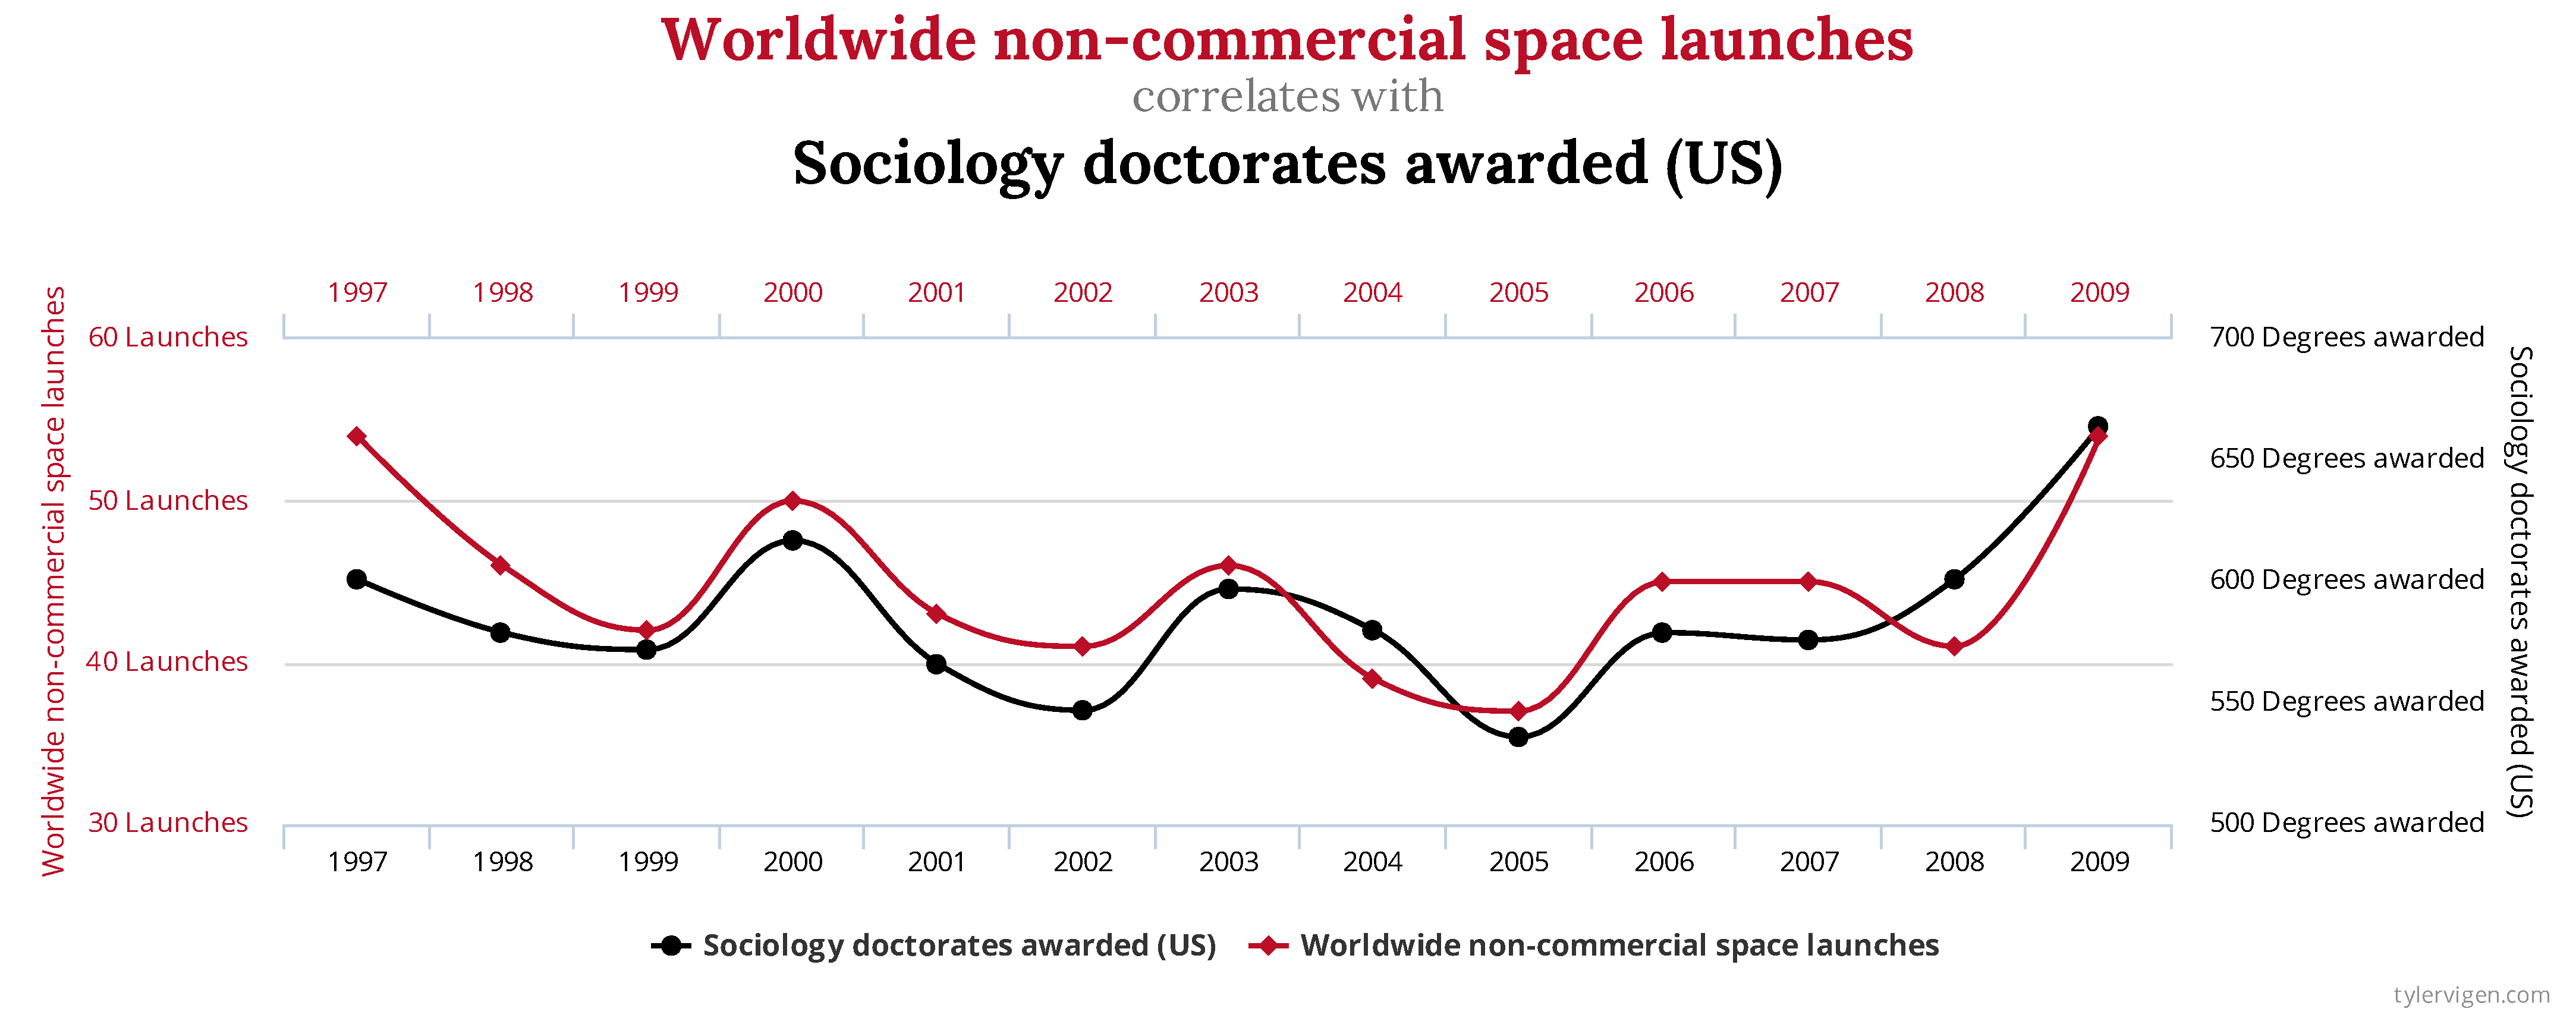
\includepdf[pages={1}]{chart_2.pdf}

\setbeamercolor{background canvas}{bg=}
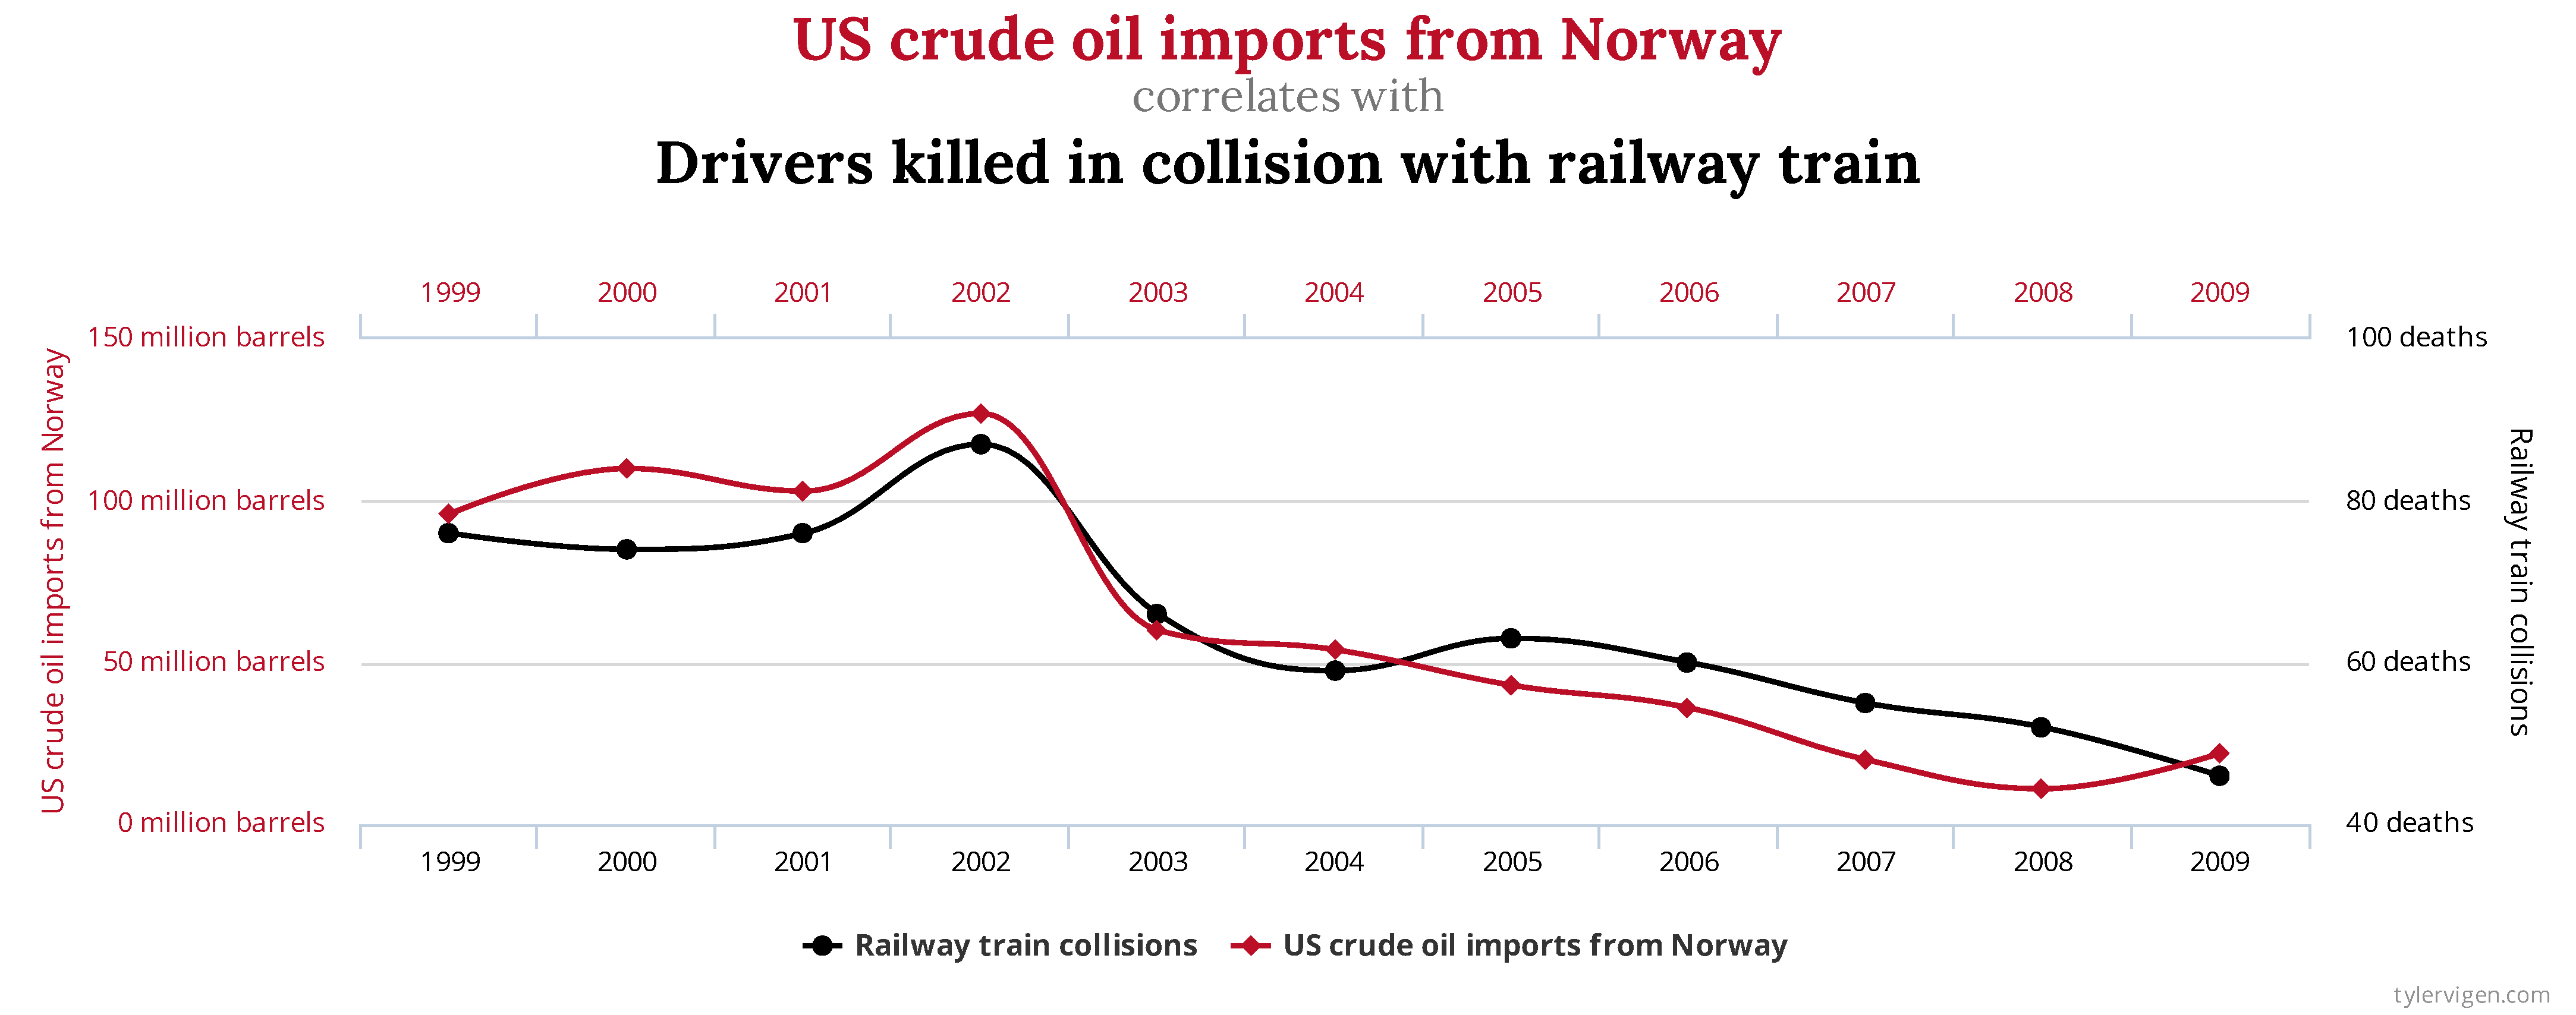
\includepdf[pages={1}]{chart_3.pdf}

\setbeamercolor{background canvas}{bg=}
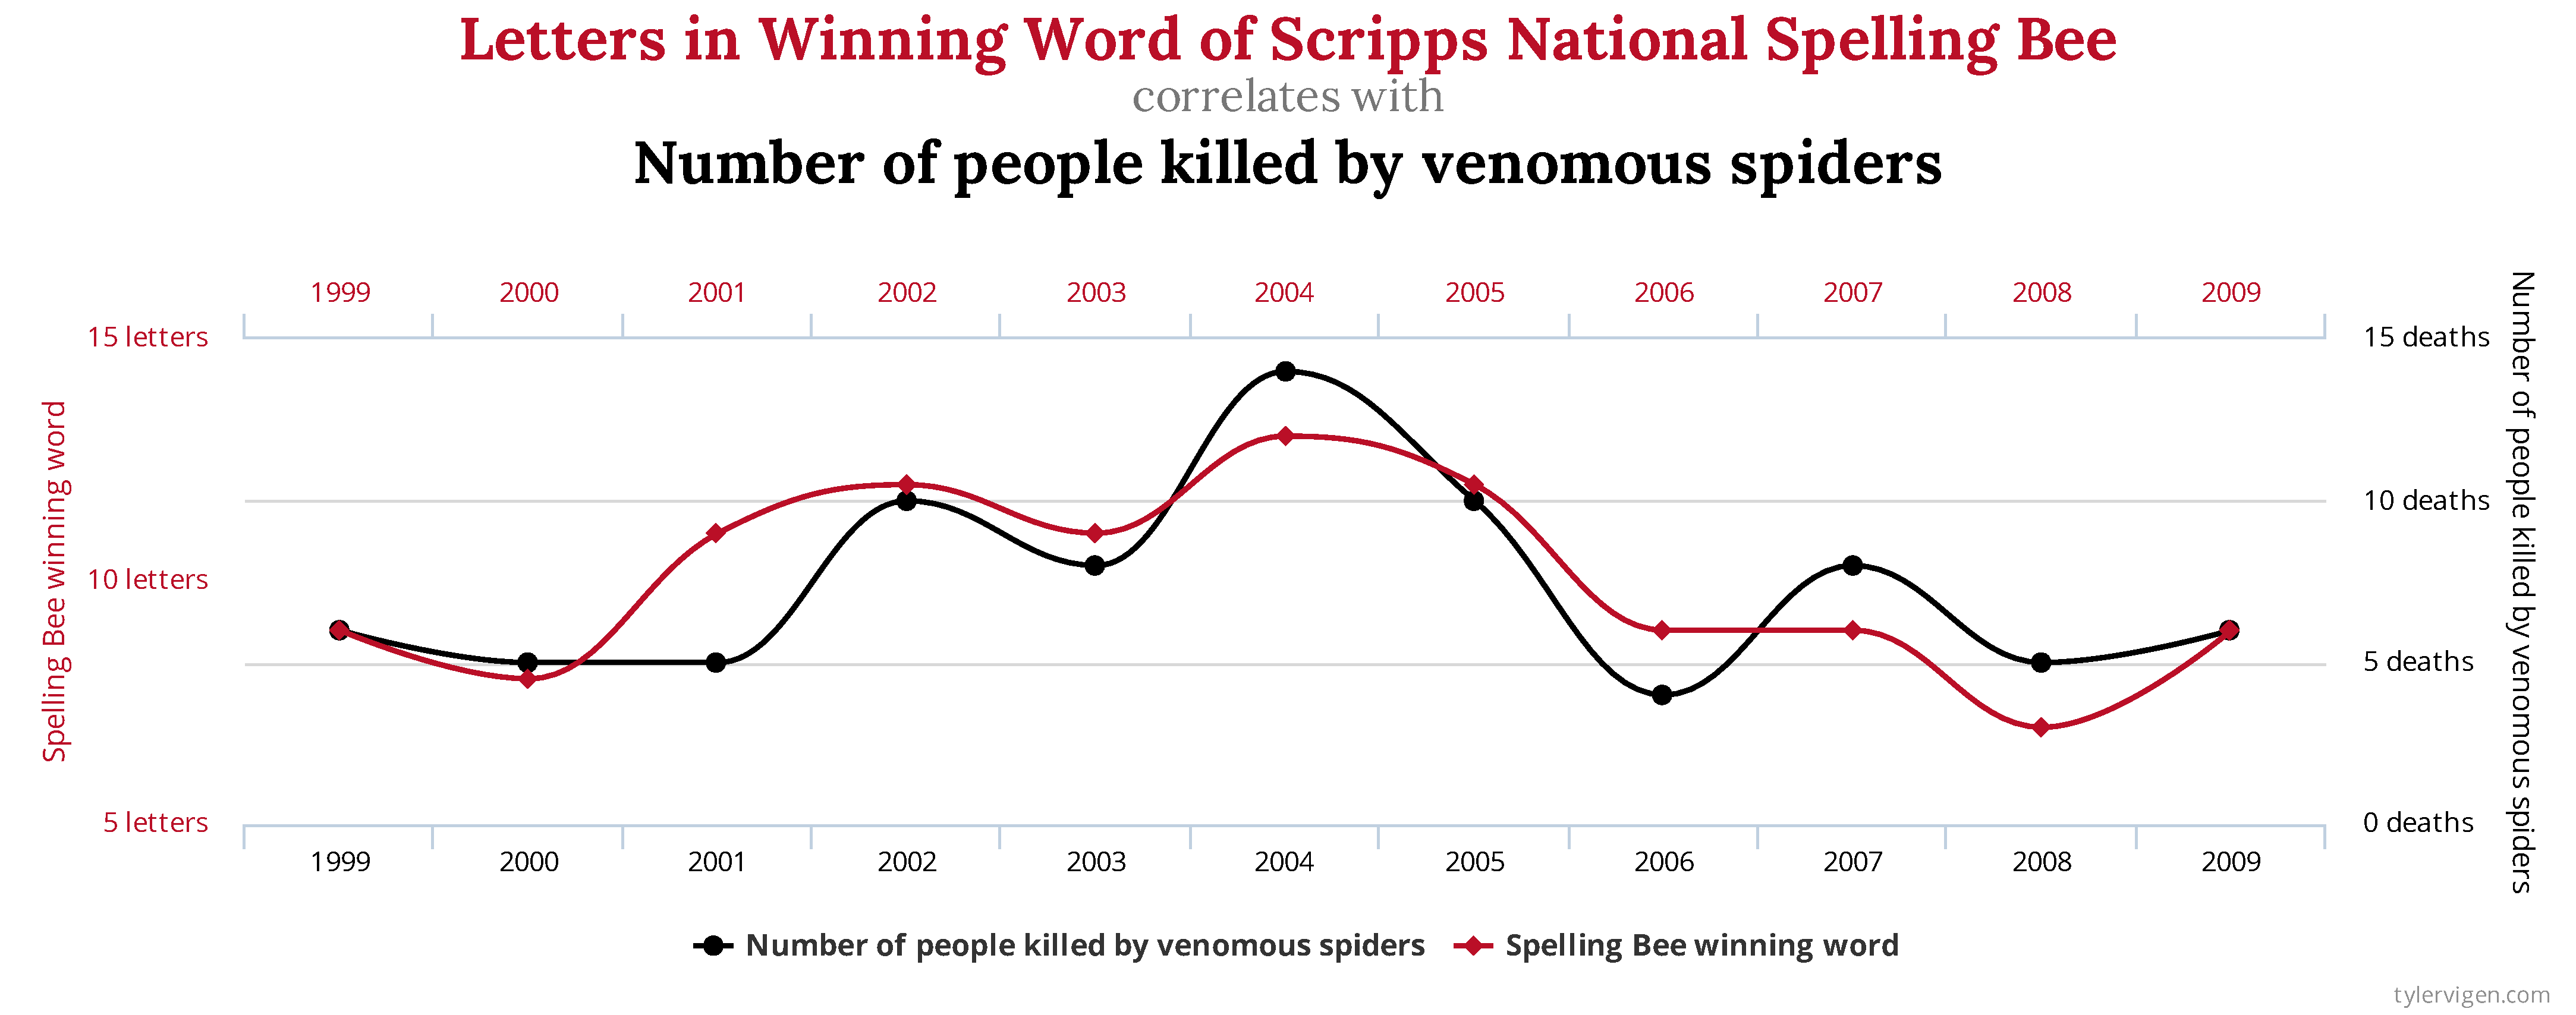
\includepdf[pages={1}]{chart_4.pdf}

\begin{frame}
\frametitle{What do political scientists \textbf{know}?}
\begin{itemize}
\item Why isn't correlation enough?
\begin{itemize}
\item For \textit{prediction} correlation is fine: If we know a country has income of US\$50,000 per capita we can confidently predict it is perceived as being less corrupt
\item But for \textit{intervention}, correlation does not help: investing to boost the economy does nothing on its own to reduce corruption
\end{itemize}
\end{itemize}
\end{frame}

\begin{frame}
\frametitle{What do political scientists \textbf{know}?}
\begin{itemize}
\item Why isn't correlation enough?
\item \textbf{The Lucas Critique}: Relationships fall apart when we intervene with policy
\begin{itemize}
\item The data shows no-one lies on their tax forms
\item So let's abandon tax checks; the government wants to save money
\item But reducing checks reduces the chances of getting caught
\item Citizens start to lie on their tax forms
\end{itemize}
\item That means we need to understand what \textit{causes} people to lie on tax forms, so we can better understand their behaviour
\end{itemize}
\end{frame}

\begin{frame}
\frametitle{What do political scientists \textbf{know}?}
\begin{itemize}
\item To accumulate knowledge, we have to ask specific types of questions:
\end{itemize}
\begin{table}[htbp]
  \centering
    \begin{tabular}{|>{\raggedright}p{5cm}|p{5cm}|}
    \toprule
    \textbf{Causes of Effects} & \textbf{Effects of Causes} \\
    \midrule
    What caused Y? & Does X cause Y?" \\
    \midrule
    Why did the United States grow faster than Bolivia in the twentieth century? & Did the more permanent colonial settlement of the United States compared to Bolivia affect their subsequent growth rates? \\
    \bottomrule
    \end{tabular}%
  \label{tab:addlabel}%
\end{table}%
\end{frame}

\begin{frame}
\frametitle{Causal Inference}
\begin{itemize}
\item A focus on a single explanatory variable $X$ requires us to clearly define this 'treatment' 
\item AND to clearly define a control
\begin{itemize}
\item What is the opposite of investing \$1bn in education?
\item No investment, or investing it elsewhere?
\end{itemize}
\item Define treatment:
\end{itemize}
\[D_i = 
\begin{cases}
1 \text{, if treated} \\
0 \text{, if not treated}
\end{cases}
\]
\end{frame}

\begin{frame}
\frametitle{Causal Inference}
\begin{itemize}
\item Defining our outcome is also crucial:
\begin{itemize}
\item Can we measure our outcome of interest?
\item Is that outcome the end of the causal chain?
\item Tempting to look at many outcomes, but the risk of cherry-picking
\begin{itemize}
\item All outcomes are probabilistic
\item If we study 20 outcomes, on average one will show a significant effect even with no real causal effect
\end{itemize}
\end{itemize}
\end{itemize}
\end{frame}

\begin{frame}
\frametitle{Causal Inference}
\begin{itemize}
\item We want to know how some variable affects another variable
\item eg. how a proportional representation electoral system affects investment in education
\begin{itemize}
\item The \textbf{treatment} is a change to a PR electoral system (vs FPTP)
\item The \textbf{outcome} is the level of (public?) investment in education
\end{itemize}
\end{itemize}
\end{frame}

\begin{frame}
\frametitle{Causal Inference}
\begin{itemize}
\item So we need a precise framework to analyze causation
\item The causal effect of treatment is how the unit's outcome differs when it is treated and not treated
\item These are the \textbf{potential outcomes} for unit $i$:
\[
Y_{Di} = 
\begin{cases}
Y_{1i}\text{   Potential Outcome if unit i treated} \\
Y_{0i}\text{   Potential Outcome if unit i not treated}
\end{cases}
\]
\item Treatment Effect $ = Y_{1i} - Y_{0i}$
\end{itemize}
\end{frame}

\begin{frame}
\frametitle{Causal Inference}
\begin{table}[htbp]
  \centering
  \caption{Potential Outcomes Example}
    \begin{tabular}{|l|p{2.4cm}|p{2.4cm}|r|}
    \hline
          & \multicolumn{1}{p{2.4cm}|}{Investment in Education if PR system} & \multicolumn{1}{p{2.4cm}|}{Investment in Education if FPTP system} &  \bigstrut\\
    \hline
          & \multicolumn{1}{l|}{$Y_1$} & \multicolumn{1}{l|}{$Y_0$} & \multicolumn{1}{l|}{Treatment Effect} \bigstrut\\
    \hline
    Brasil & 8     & 4     & 4 \bigstrut\\
    \hline
    Argentina & 10    & 7     & 3 \bigstrut\\
    \hline
    Bolivia & 2     & 4     & -2 \bigstrut\\
    \hline
    Colombia & 11    & 11    & 0 \bigstrut\\
    \hline
    Peru & 6     & 2     & 4 \bigstrut\\
    \hline
    \end{tabular}%
  \label{tab:addlabel}%
\end{table}%
\end{frame}

\begin{frame}
\frametitle{Causal Inference}
\begin{itemize}
\item \textbf{The Fundamental Problem of Causal Inference}
\begin{itemize}
\item No units can receive \textbf{both} treatment and control
\item So we can never observe both $Y_1$ and $Y_0$ for the same unit
\end{itemize}
\end{itemize}
\end{frame}

\begin{frame}
\frametitle{Causal Inference}
\footnotesize
\begin{table}[htbp]
  \centering
  \caption{Potential Outcomes Example}
    \begin{tabular}{|p{1.8cm}|p{2.2cm}|p{2.2cm}|p{1.8cm}|r|}
    \hline
          & \multicolumn{1}{p{1.8cm}|}{PR System?} & \multicolumn{1}{p{2.2cm}|}{Investment in Education if PR system} & \multicolumn{1}{p{2.2cm}|}{Investment in Education if FPTP system} &  \bigstrut\\
    \hline
          & \multicolumn{1}{p{1.8cm}|}{$D_i$} & \multicolumn{1}{p{2.2cm}|}{$Y_1$} & \multicolumn{1}{p{2.2cm}|}{$Y_0$} & \multicolumn{1}{p{1.8cm}|}{Treatment Effect} \bigstrut\\
    \hline
    Brasil & 1 & 8     & ?      & ? \bigstrut\\
    \hline
    Argentina & 1 & 10    & ?      & ? \bigstrut\\
    \hline
    Bolivia & 0 & ?     & 4     & ? \bigstrut\\
    \hline
    Colombia & 0 &  ?   & 11    & ? \bigstrut\\
    \hline
    Peru & 0 & ?     & 2     & ? \bigstrut\\
    \hline
    \end{tabular}%
  \label{tab:addlabel}%
\end{table}%
\normalsize
\end{frame}

\begin{frame}
\frametitle{Causal Inference}
\begin{itemize}
\item We can't even look at the change in countries that switch to a PR system
\begin{itemize}
\item What if \textbf{all} countries had started to invest more in education at the same time, for different reasons?
\item The potential outcome for Country X in time 1 is different to at time 2
\end{itemize}
\end{itemize}
\end{frame}

\begin{frame}
\frametitle{Causal Inference}
\begin{itemize}
\item So we need to consider the \textbf{counterfactual} - what would have happened if the country had \textbf{not} switched to a PR system?
\begin{itemize}
\item This is \textbf{impossible} to know
\item We can only estimate the effect by comparing \textbf{across} units in some way
\item That is why we are doing causal \textbf{inference}, not causal proof
\end{itemize}
\end{itemize}
\end{frame}

\begin{frame}
\frametitle{Causal Inference}
\begin{itemize}
\item Which comparisons to make? 
\item Control units can never be perfect substitutes
\item Causal Inference is all about identifying a \textbf{plausible counterfactual}
\begin{itemize}
\item Plausible means that the potential outcomes of the control unit are likely to be the same as those of the treated unit
\end{itemize}
\end{itemize}
\end{frame}

\begin{frame}
\frametitle{Causal Inference}
\begin{itemize}
\item The comparability of treatment and control units depends on \textit{how} they got to be treated
\begin{itemize}
\item On the \textbf{Treatment Assignment Mechanism}
\end{itemize}
\item If we 'treated' an outlier like the Galapagos Islands, could we find a comparable control unit?
\item Comparisons are easier where the \textbf{Treatment Assignment Mechanism is independent of potential outcomes}
\begin{itemize}
\item This makes it more likely that potential outcomes are 'balanced' and comparable
\end{itemize}
\end{itemize}
\end{frame}

\begin{frame}
\frametitle{Causal Inference}
\begin{itemize}
\item Types of Research Design:
\end{itemize}
\begin{table}[htbp]
  \centering
  \caption{Add caption}
    \begin{tabular}{|>{\raggedright}p{5cm}|p{5cm}|p{5cm}|}
    \toprule
          & Researcher controls the treatment assignment & Treatment assignment mechanism likely to create comparable potential outcomes \\
    \midrule
    Controlled Experiments & Yes   & Yes \\
    \midrule
    Natural Experiments & No    & Yes \\
    \midrule
    Observable Studies & No    & No \\
    \bottomrule
    \end{tabular}%
  \label{tab:addlabel}%
\end{table}%
\end{frame}

\begin{frame}
\frametitle{Problems with Observational Data}
\begin{itemize}
\item Observational Studies
\begin{itemize}
\item Household surveys
\item Simple regression on secondary data
\item Interviews of a random sample
\end{itemize}
\end{itemize}
\end{frame}

\begin{frame}
\frametitle{Problems with Observational Data}
\begin{itemize}
\item We do not know what the treatment assignment mechanism was
\begin{itemize}
\item Which units were treated and why?
\end{itemize}
\item Treatment assignment is unlikely to create comparable potential outcomes
\begin{itemize}
\item Which units might be appropriate counterfactuals?
\end{itemize}
\end{itemize}
\end{frame}

\begin{frame}
\frametitle{Problems with Observational Data}
\begin{itemize}
\item With complete information on potential outcomes, calculating treatment effects is trivial
\end{itemize}
\begin{table}[htbp]
  \centering
  \caption{Calculating Treatment Effects}
    \begin{tabular}{|l|r|r|r|r|r|}
    \hline
          & \multicolumn{1}{l|}{D} & \multicolumn{1}{l|}{$Y_1$} & \multicolumn{1}{l|}{$Y_0$} & \multicolumn{1}{l|}{$Y_i$} & \multicolumn{1}{l|}{Real Effect, $Y_1 - Y_0$} \bigstrut\\
    \hline
    A     & 1     & 7     & 4     & 7     & 3 \bigstrut\\
    \hline
    B     & 0     & 9     & 5     & 5     & 4 \bigstrut\\
    \hline
    C     & 0     & 4     & 4     & 4     & 0 \bigstrut\\
    \hline
    D     & 1     & 4     & 3     & 4     & 1 \bigstrut\\
    \hline \pause
    $E(Y_1)=$ & & 6 & & \bigstrut\\
    \hline
    $E(Y_0)=$ & &  & 4& \bigstrut\\
    \hline
    \end{tabular}%
  \label{tab:addlabel}%
\end{table}%
\begin{itemize}
\item $ATE = E(Y_1-Y_0) = 8/4 = 2$
\item $ATE = E(Y_1) - E(Y_0) = 6 - 4 = 2$
\end{itemize}
\end{frame}

\begin{frame}
\frametitle{Problems with Observational Data}
\begin{itemize}
\item From observed outcomes can we calculate an Average Treatment Effect?
\end{itemize}
\begin{table}[htbp]
  \centering
  \caption{Calculating Treatment Effects}
    \begin{tabular}{|l|r|r|r|r|r|}
    \hline
          & \multicolumn{1}{l|}{D} & \multicolumn{1}{l|}{$Y_1$} & \multicolumn{1}{l|}{$Y_0$} & \multicolumn{1}{l|}{$Y_i$} & \multicolumn{1}{l|}{Real Effect, $Y_1 - Y_0$} \bigstrut\\
    \hline
    A     & 1     & \cellcolor{teal}7     & ?     & 7     & ? \bigstrut\\
    \hline
    B     & 0     & ?     & \cellcolor{teal}5     & 5     & ? \bigstrut\\
    \hline
    C     & 0     & ?     & \cellcolor{teal}4     & 4     & ? \bigstrut\\
    \hline
    D     & 1     & \cellcolor{teal}4     & ?     & 4     & ? \bigstrut\\
    \hline \pause
    $E(Y_1)=$ & & 5.5 & & \bigstrut\\
    \hline
    $E(Y_0)=$ & &  & 4.5 & \bigstrut\\
    \hline
    \end{tabular}%
  \label{tab:addlabel}%
\end{table}%
\end{frame}

\begin{frame}
\frametitle{Problems with Observational Data}
\begin{itemize}
\item If we use the control units as counterfactuals...
\item Average Treatment Effect:
\begin{align}
ATE &=& E(Y_1) - E(Y_0) \\
&=& 5.5 - 4.5 \\
&=& 1
\end{align}
\item Half the true treatment effect
\pause
\item Why?
\pause
\begin{itemize}
\item The units that got treated had lower $Y_1$
\item The units that were controls had higher $Y_0$
\pause
\item The 'stand-in' counterfactuals were wrong
\end{itemize}
\end{itemize}
\end{frame}

\begin{frame}
\frametitle{Problems with Observational Data}
\begin{itemize}
\item The bias in units' potential outcomes depends on which units get treated and which ones don't
\item In observational studies, we have very little protection against causal critiques
\begin{enumerate}
\item Reverse Causation
\item Omitted variable bias (confounding)
\item Selection bias
\end{enumerate}
\end{itemize}
\end{frame}

\begin{frame}
\frametitle{Reverse Causation}
\begin{itemize}
\item Wealthier countries are more likely to be democracies
\begin{itemize}
\item But does wealth create democracy?
\item Or democracy create wealth?
\end{itemize}
\item We cannot tell from the correlation alone
\item Both may be true
\end{itemize}
\end{frame}

\begin{frame}
\frametitle{Reverse Causation}
\begin{knitrout}
\definecolor{shadecolor}{rgb}{0.969, 0.969, 0.969}\color{fgcolor}
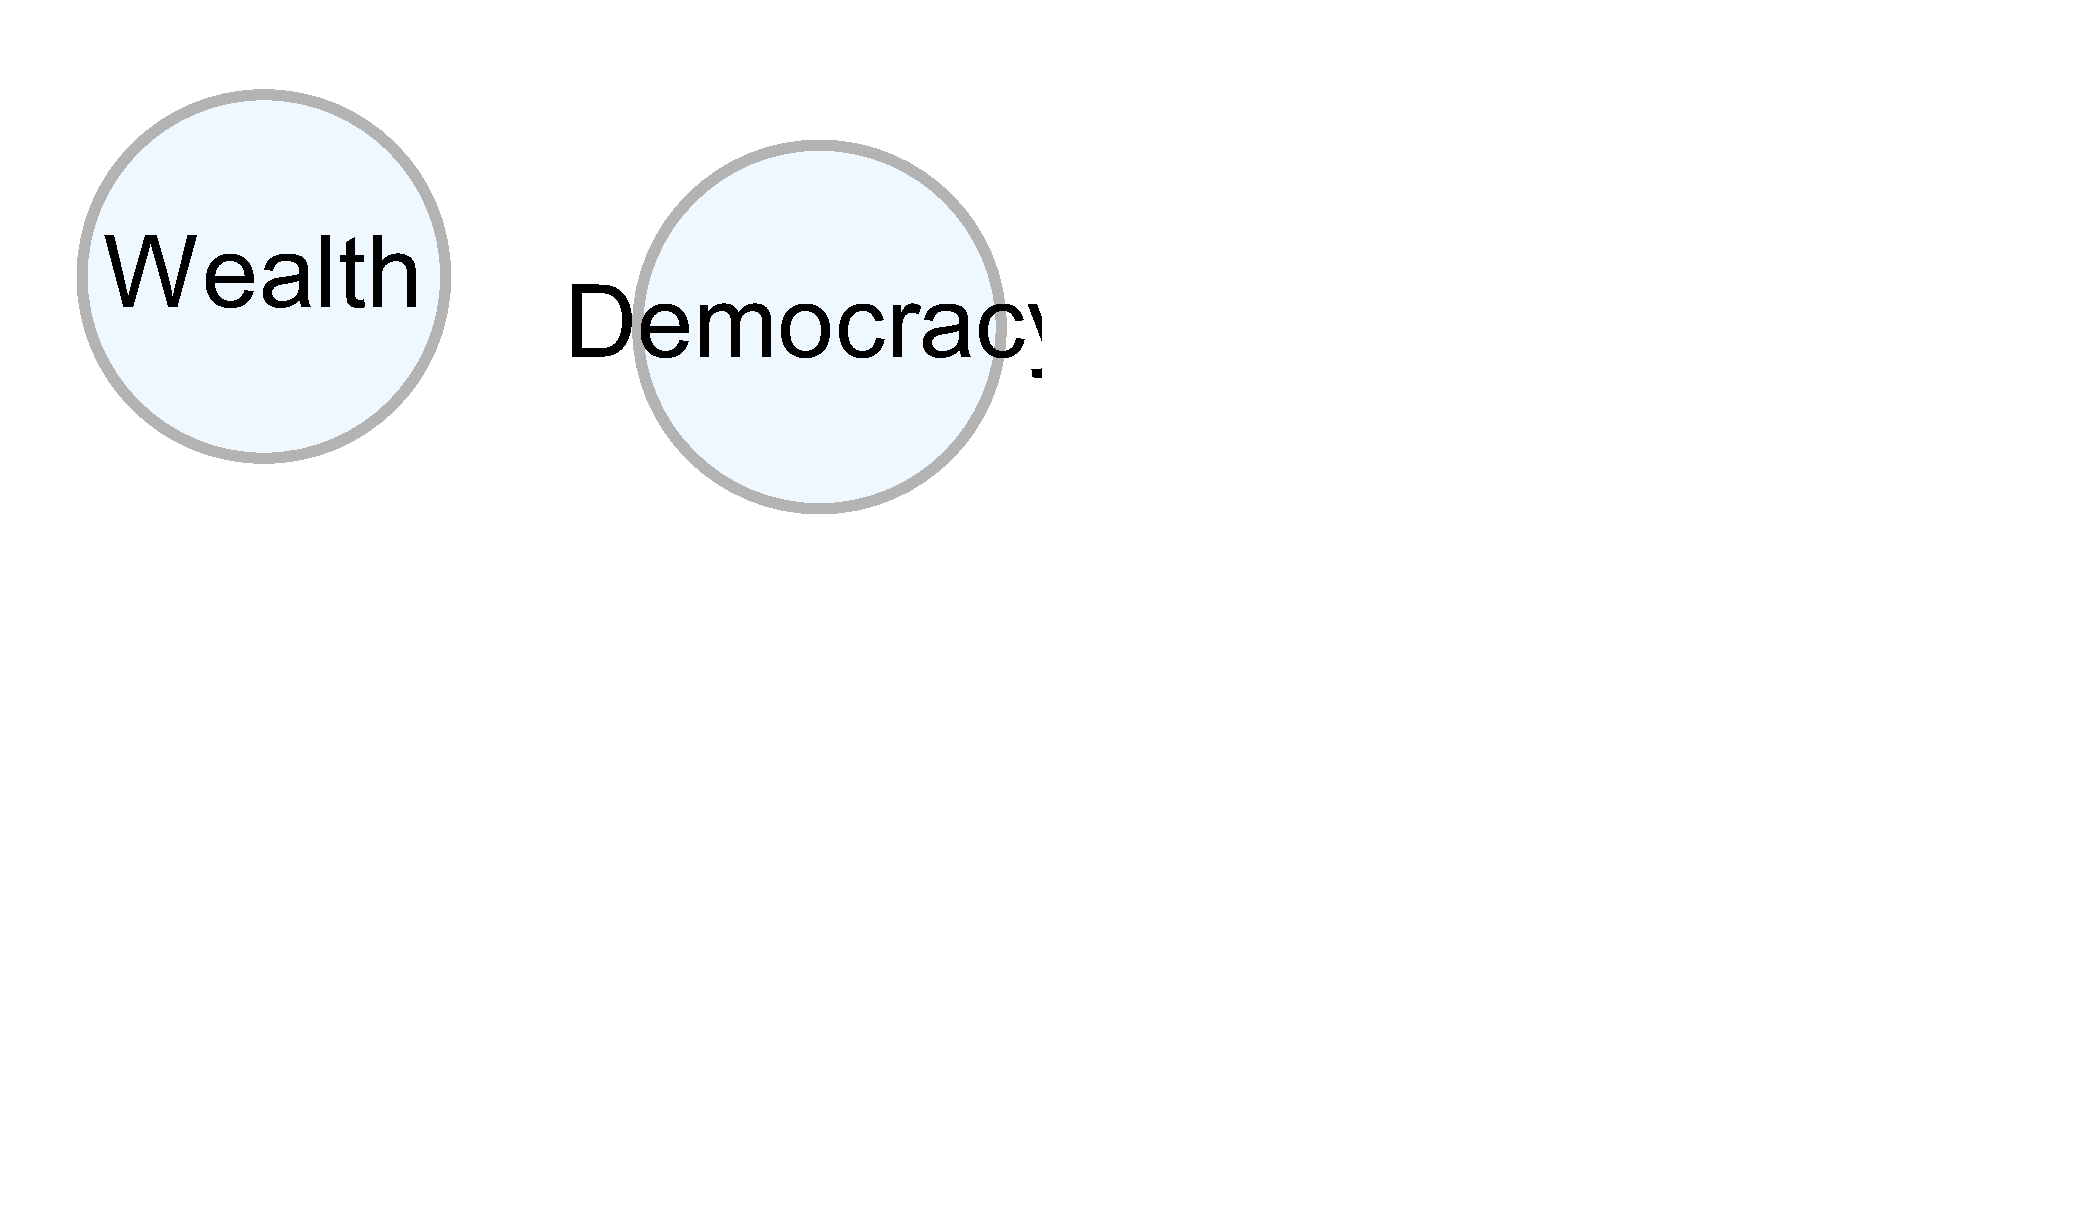
\includegraphics[width=\maxwidth]{figure/unnamed-chunk-1-1} 

\end{knitrout}
\end{frame}

\begin{frame}
\frametitle{Reverse Causation}
\begin{knitrout}
\definecolor{shadecolor}{rgb}{0.969, 0.969, 0.969}\color{fgcolor}
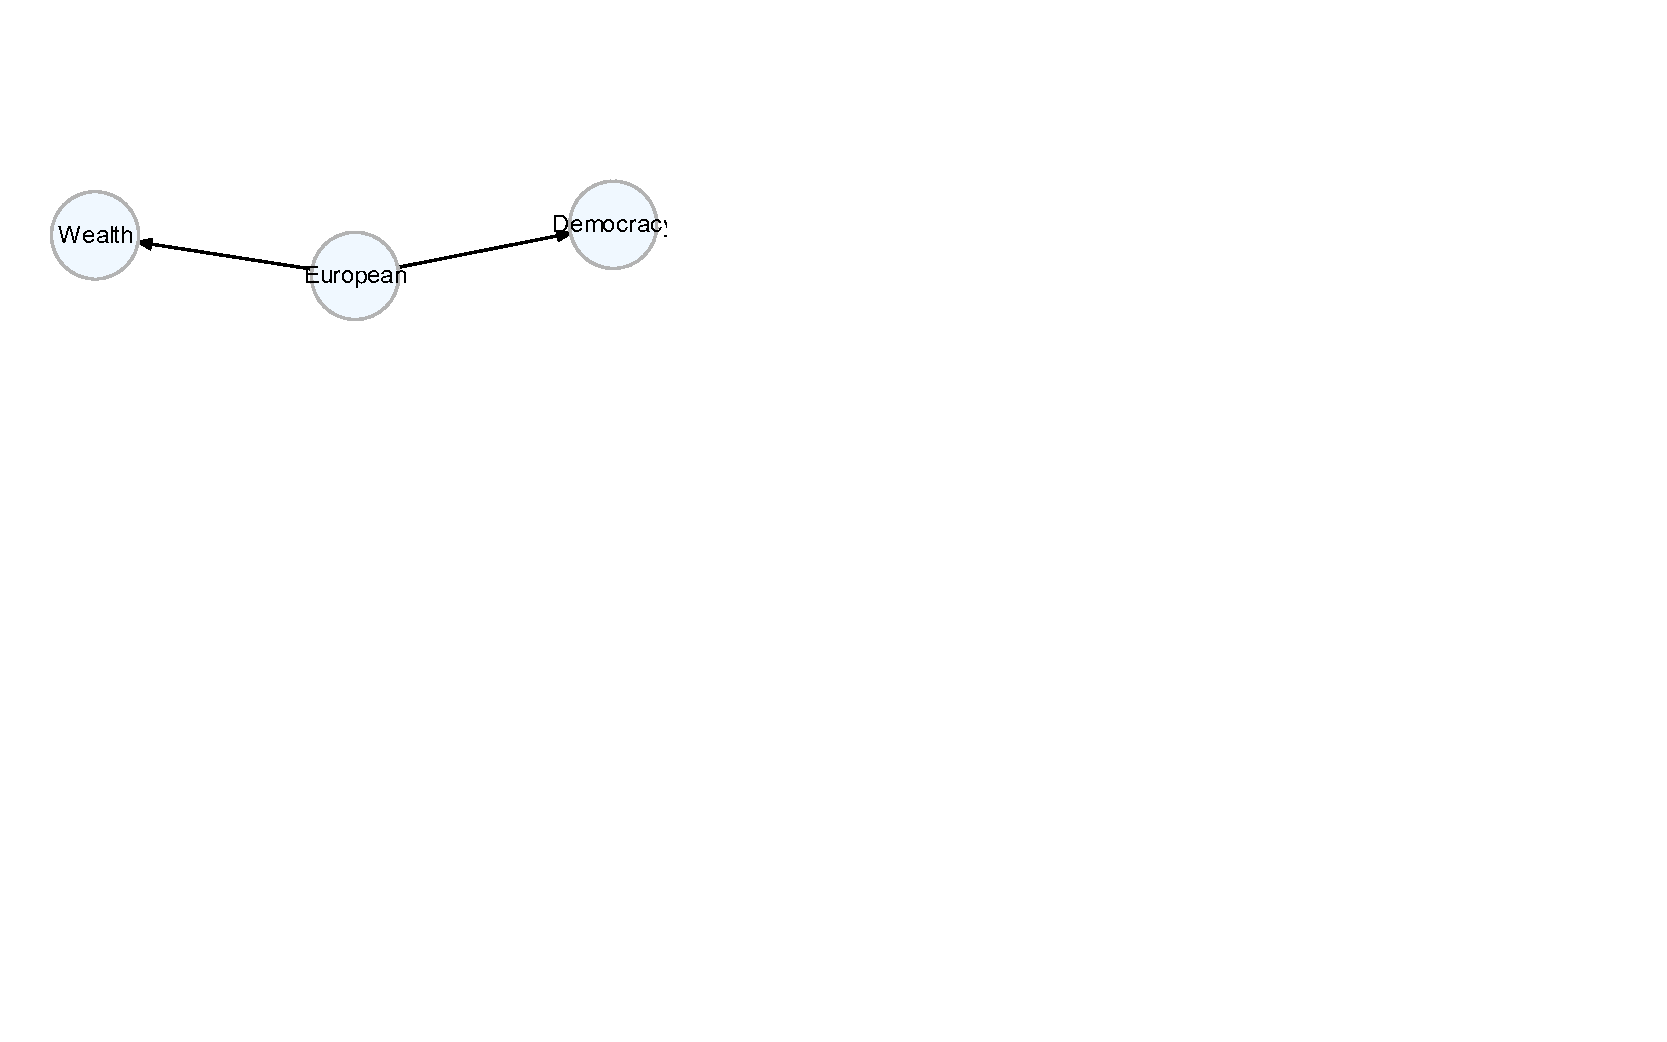
\includegraphics[width=\maxwidth]{figure/unnamed-chunk-2-1} 

\end{knitrout}
\end{frame}

\begin{frame}
\frametitle{Reverse Causation}
\begin{knitrout}
\definecolor{shadecolor}{rgb}{0.969, 0.969, 0.969}\color{fgcolor}
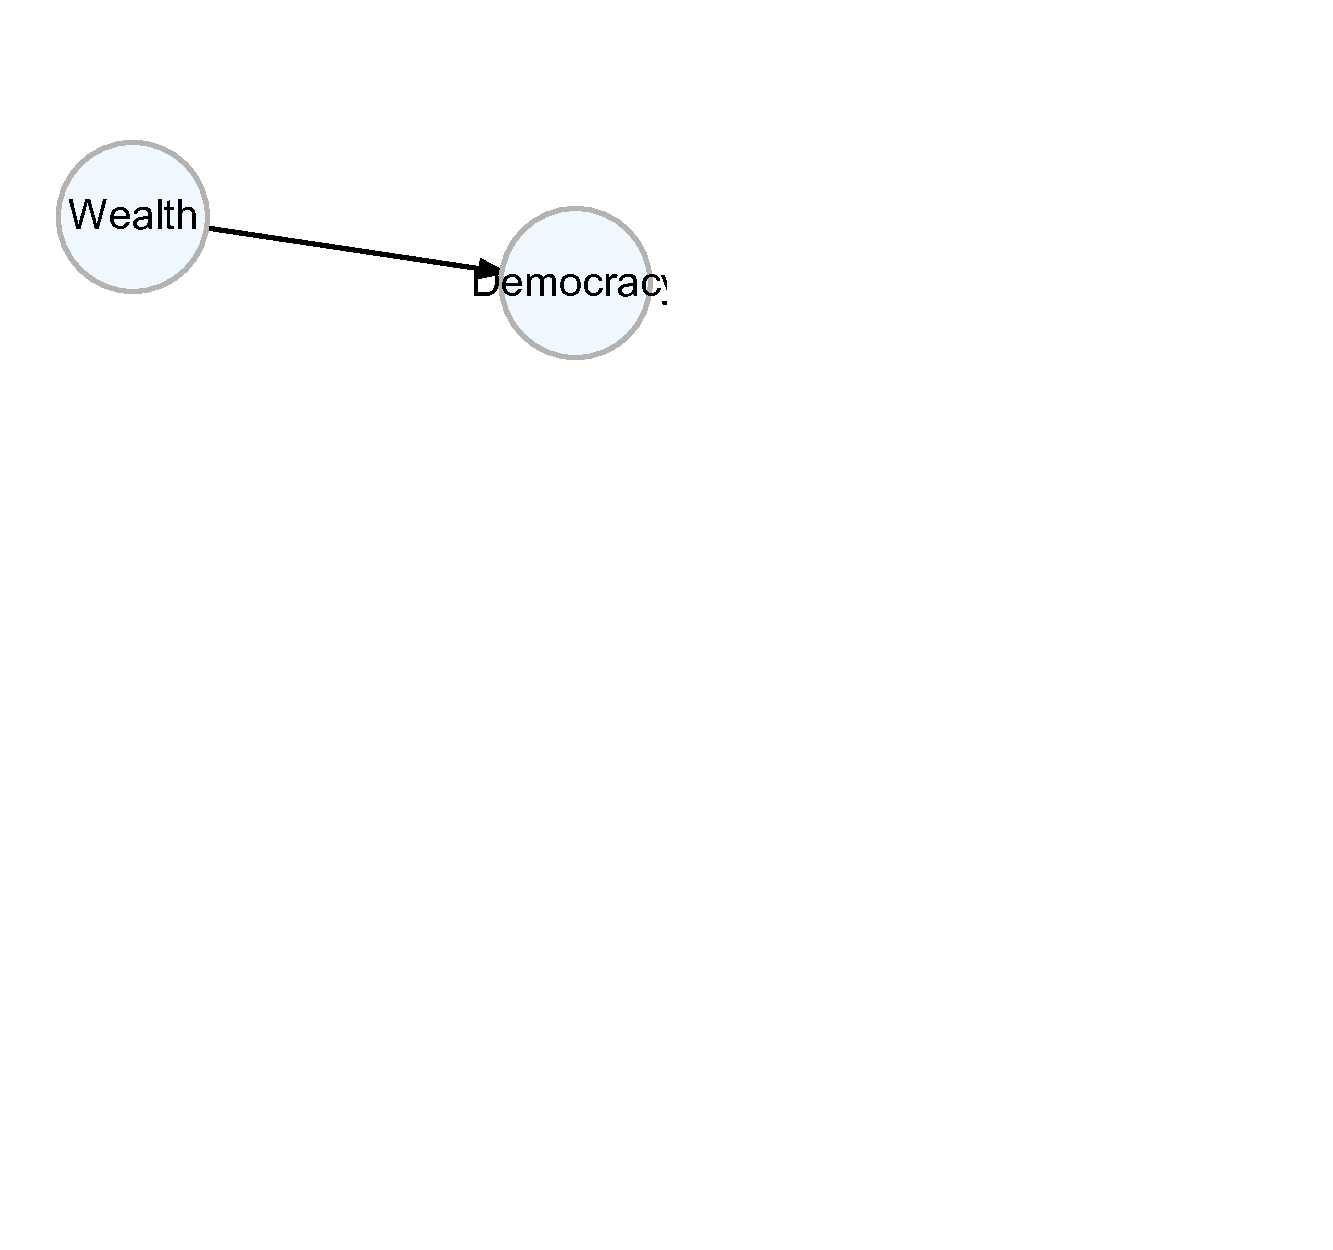
\includegraphics[width=\maxwidth]{figure/unnamed-chunk-3-1} 

\end{knitrout}
\end{frame}

\begin{frame}
\frametitle{Reverse Causation}
\begin{itemize}
\item Where treatment has $no$ effect
\end{itemize}
\begin{table}[htbp]
  \centering
  \caption{Treatment Assignment by Covariate}
    \begin{tabular}{|l|r|r|l|r|l|}
    \hline
          &  \multicolumn{1}{l|}{D} & \multicolumn{1}{l|}{$Y_1$} & $Y_0$  & \multicolumn{1}{l|}{$Y_i$} & Real Effect \bigstrut\\
    \hline
    A     & 0     & \multicolumn{1}{l|}{7} & \multicolumn{1}{r|}{\cellcolor{teal}7} & 7     & 0 \bigstrut\\
    \hline
    B     & 0     & \multicolumn{1}{l|}{9} & \multicolumn{1}{r|}{\cellcolor{teal}9} & 9     & 0 \bigstrut\\
    \hline
    C     &  1     & \cellcolor{teal}4     & 4     & 4     & 0 \bigstrut\\
    \hline
    D     & 1     & \cellcolor{teal}4     & 4     & 4     & 0 \bigstrut\\
    \hline\pause
    $E(Y_1)=$ & & 4 & & \bigstrut\\
    \hline
    $E(Y_0)=$ &  & & 4 & \bigstrut\\
    \hline
    \end{tabular}%
  \label{tab:addlabel}%
\end{table}%
\begin{itemize}
\pause
\item ATE = 4 - 4 = 0. There is no effect. 
\item The (negative) correlation between $D$ and $Y$ is because $Y$ \textbf{causes} $D$
\end{itemize}
\end{frame}

\begin{frame}
\frametitle{Omitted Variable Bias}
\begin{itemize}
\item Wealthier countries are more likely to be democracies
\begin{itemize}
\item But wealthier countries are more likely to be European
\item And democracies are more likely to be European
\end{itemize}
\item Maybe the correlation just reflects the fact that European countries are 'different'?
\end{itemize}
\end{frame}

\begin{frame}
\frametitle{Omitted Variable Bias}
\begin{knitrout}
\definecolor{shadecolor}{rgb}{0.969, 0.969, 0.969}\color{fgcolor}
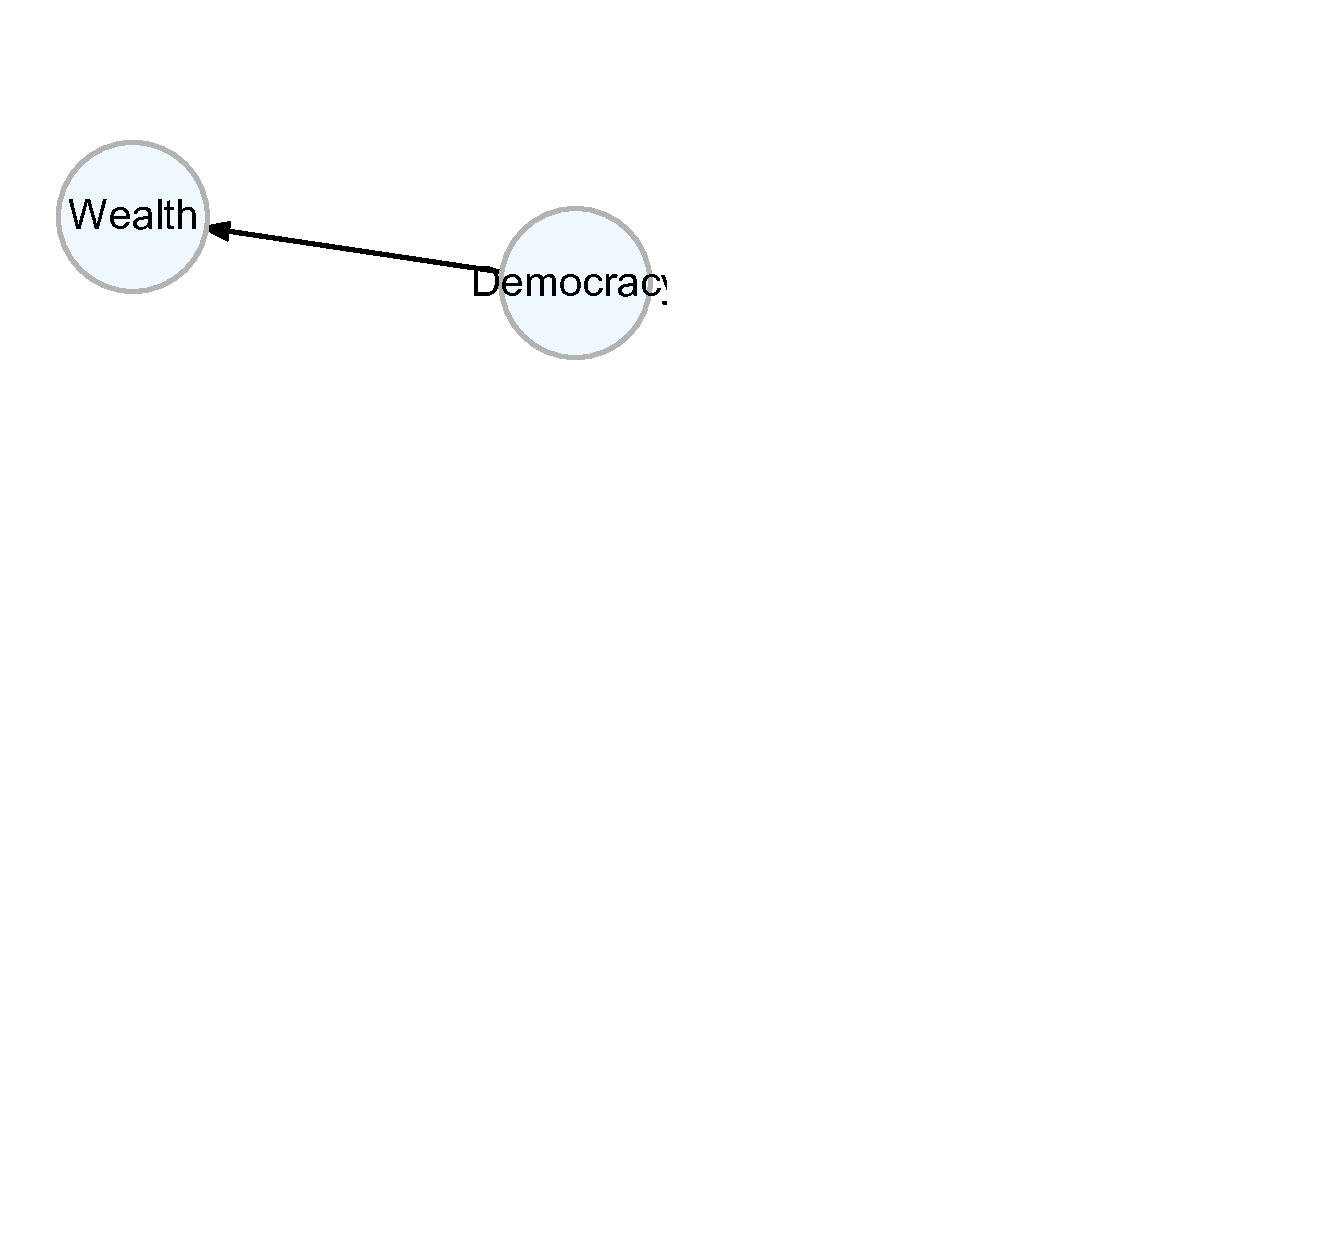
\includegraphics[width=\maxwidth]{figure/unnamed-chunk-4-1} 

\end{knitrout}
\end{frame}

\begin{frame}
\frametitle{Omitted Variable Bias}
\begin{knitrout}
\definecolor{shadecolor}{rgb}{0.969, 0.969, 0.969}\color{fgcolor}
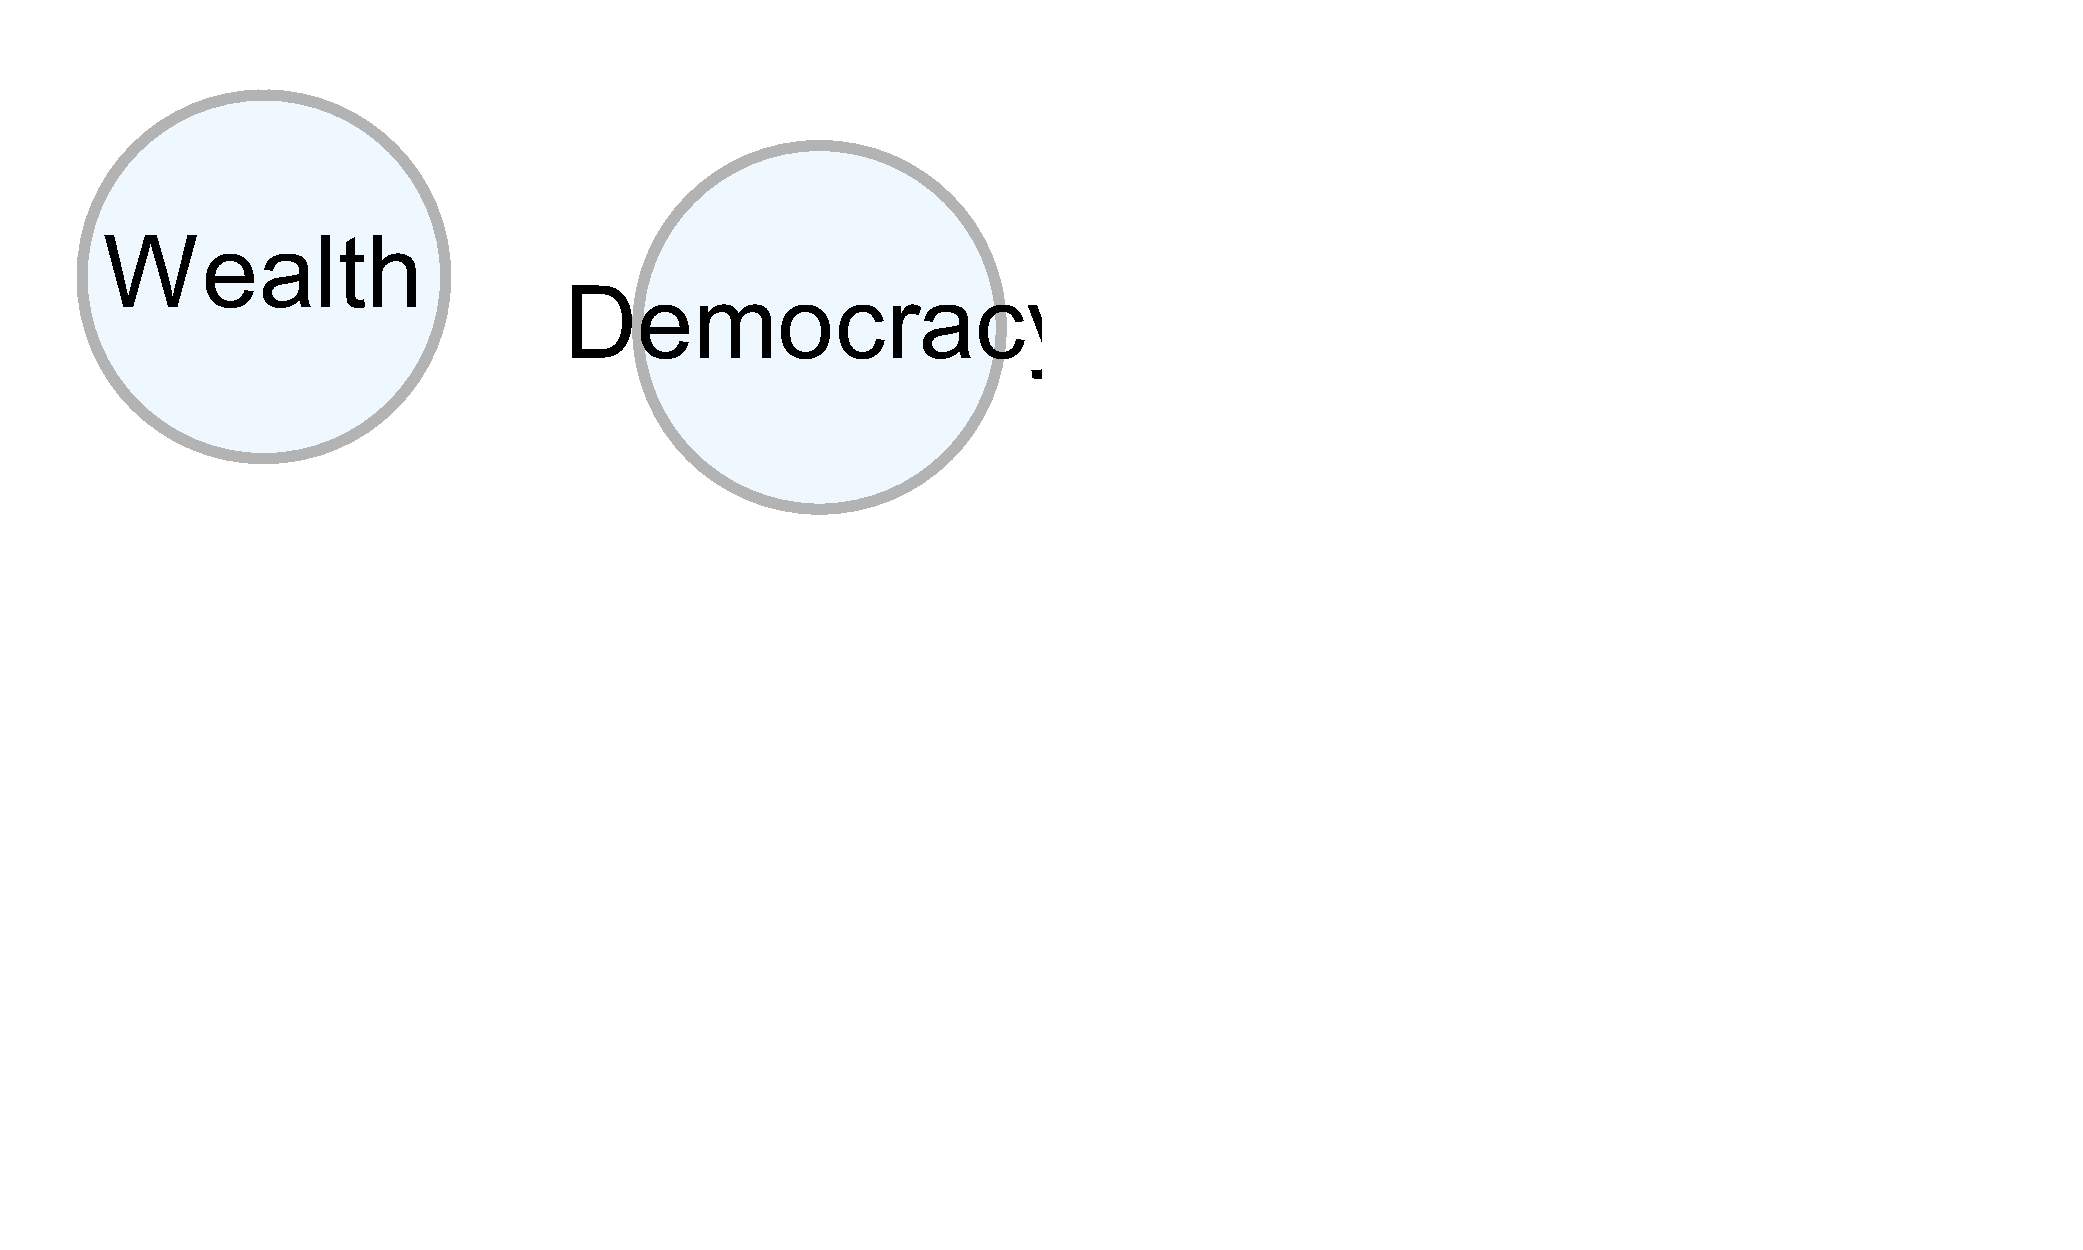
\includegraphics[width=\maxwidth]{figure/unnamed-chunk-5-1} 

\end{knitrout}
\end{frame}


\begin{frame}
\frametitle{Omitted Variable Bias}
\begin{itemize}
\item Imagine a treatment assignment mechanism where all women get treated
\end{itemize}
\begin{table}[htbp]
  \centering
  \caption{Treatment Assignment by Covariate}
    \begin{tabular}{|l|l|r|r|l|r|l|}
    \hline
          & X     & \multicolumn{1}{l|}{D} & \multicolumn{1}{l|}{$Y_1$} & $Y_0$  & \multicolumn{1}{l|}{$Y_i$} & Real Effect \bigstrut\\
    \hline
    A     & Man   & 0     & \multicolumn{1}{l|}{7} & \multicolumn{1}{r|}{\cellcolor{teal}4} & 4     & 3 \bigstrut\\
    \hline
    B     & Man   & 0     & \multicolumn{1}{l|}{9} & \multicolumn{1}{r|}{\cellcolor{teal}5} & 5     & 4 \bigstrut\\
    \hline
    C     & Woman & 1     & \cellcolor{teal}4     & 4     & 4     & 0 \bigstrut\\
    \hline
    D     & Woman & 1     & \cellcolor{teal}4     & 3     & 4     & 1 \bigstrut\\
    \hline\pause
    $E(Y_1)=$ & & & 4 & & \bigstrut\\
    \hline
    $E(Y_0)=$ & &  & & 4.5 & \bigstrut\\
    \hline
    \end{tabular}%
  \label{tab:addlabel}%
\end{table}%
\begin{itemize}
\pause
\item ATE = 4 - 4.5 = -0.5
\item This is \textbf{confounding} or an \textbf{omitted variable} - another variable affects both treatment and potential outcomes
\end{itemize}
\end{frame}

\begin{frame}
\frametitle{Self-Selecion Bias}
\begin{itemize}
\item Wealthier countries are more likely to be democracies
\begin{itemize}
\item But wealthy autocracies and poor democracies do not like to report data
\item So we cannot compare them
\item Only wealthy democracies 'self-select' into our sample
\end{itemize}
\end{itemize}
\end{frame}

\begin{frame}
\frametitle{Self-Selection Bias}
\begin{knitrout}
\definecolor{shadecolor}{rgb}{0.969, 0.969, 0.969}\color{fgcolor}
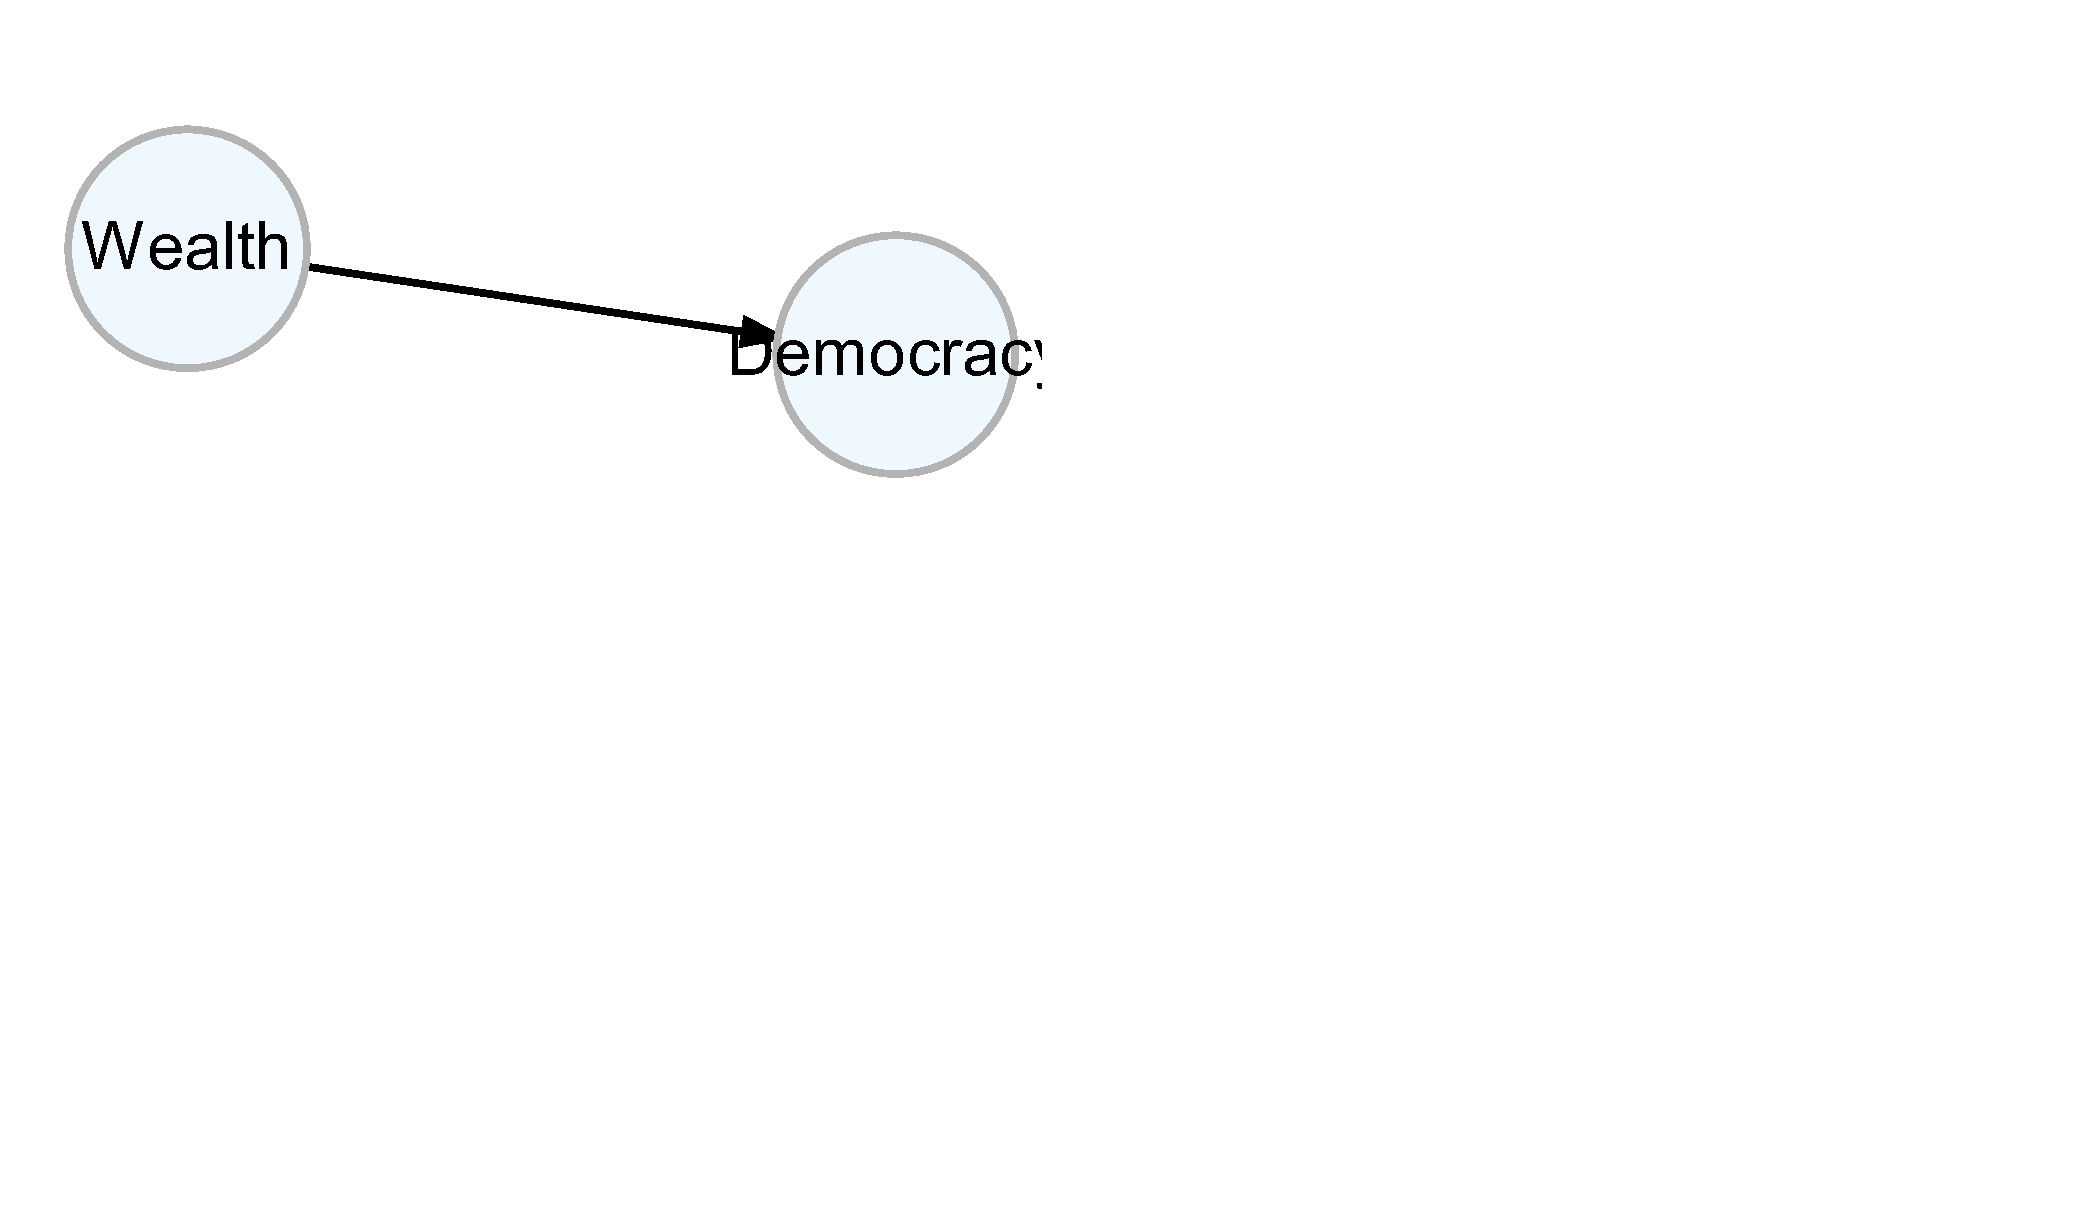
\includegraphics[width=\maxwidth]{figure/unnamed-chunk-6-1} 

\end{knitrout}
\end{frame}

\begin{frame}
\frametitle{Self-Selection Bias}
\begin{knitrout}
\definecolor{shadecolor}{rgb}{0.969, 0.969, 0.969}\color{fgcolor}
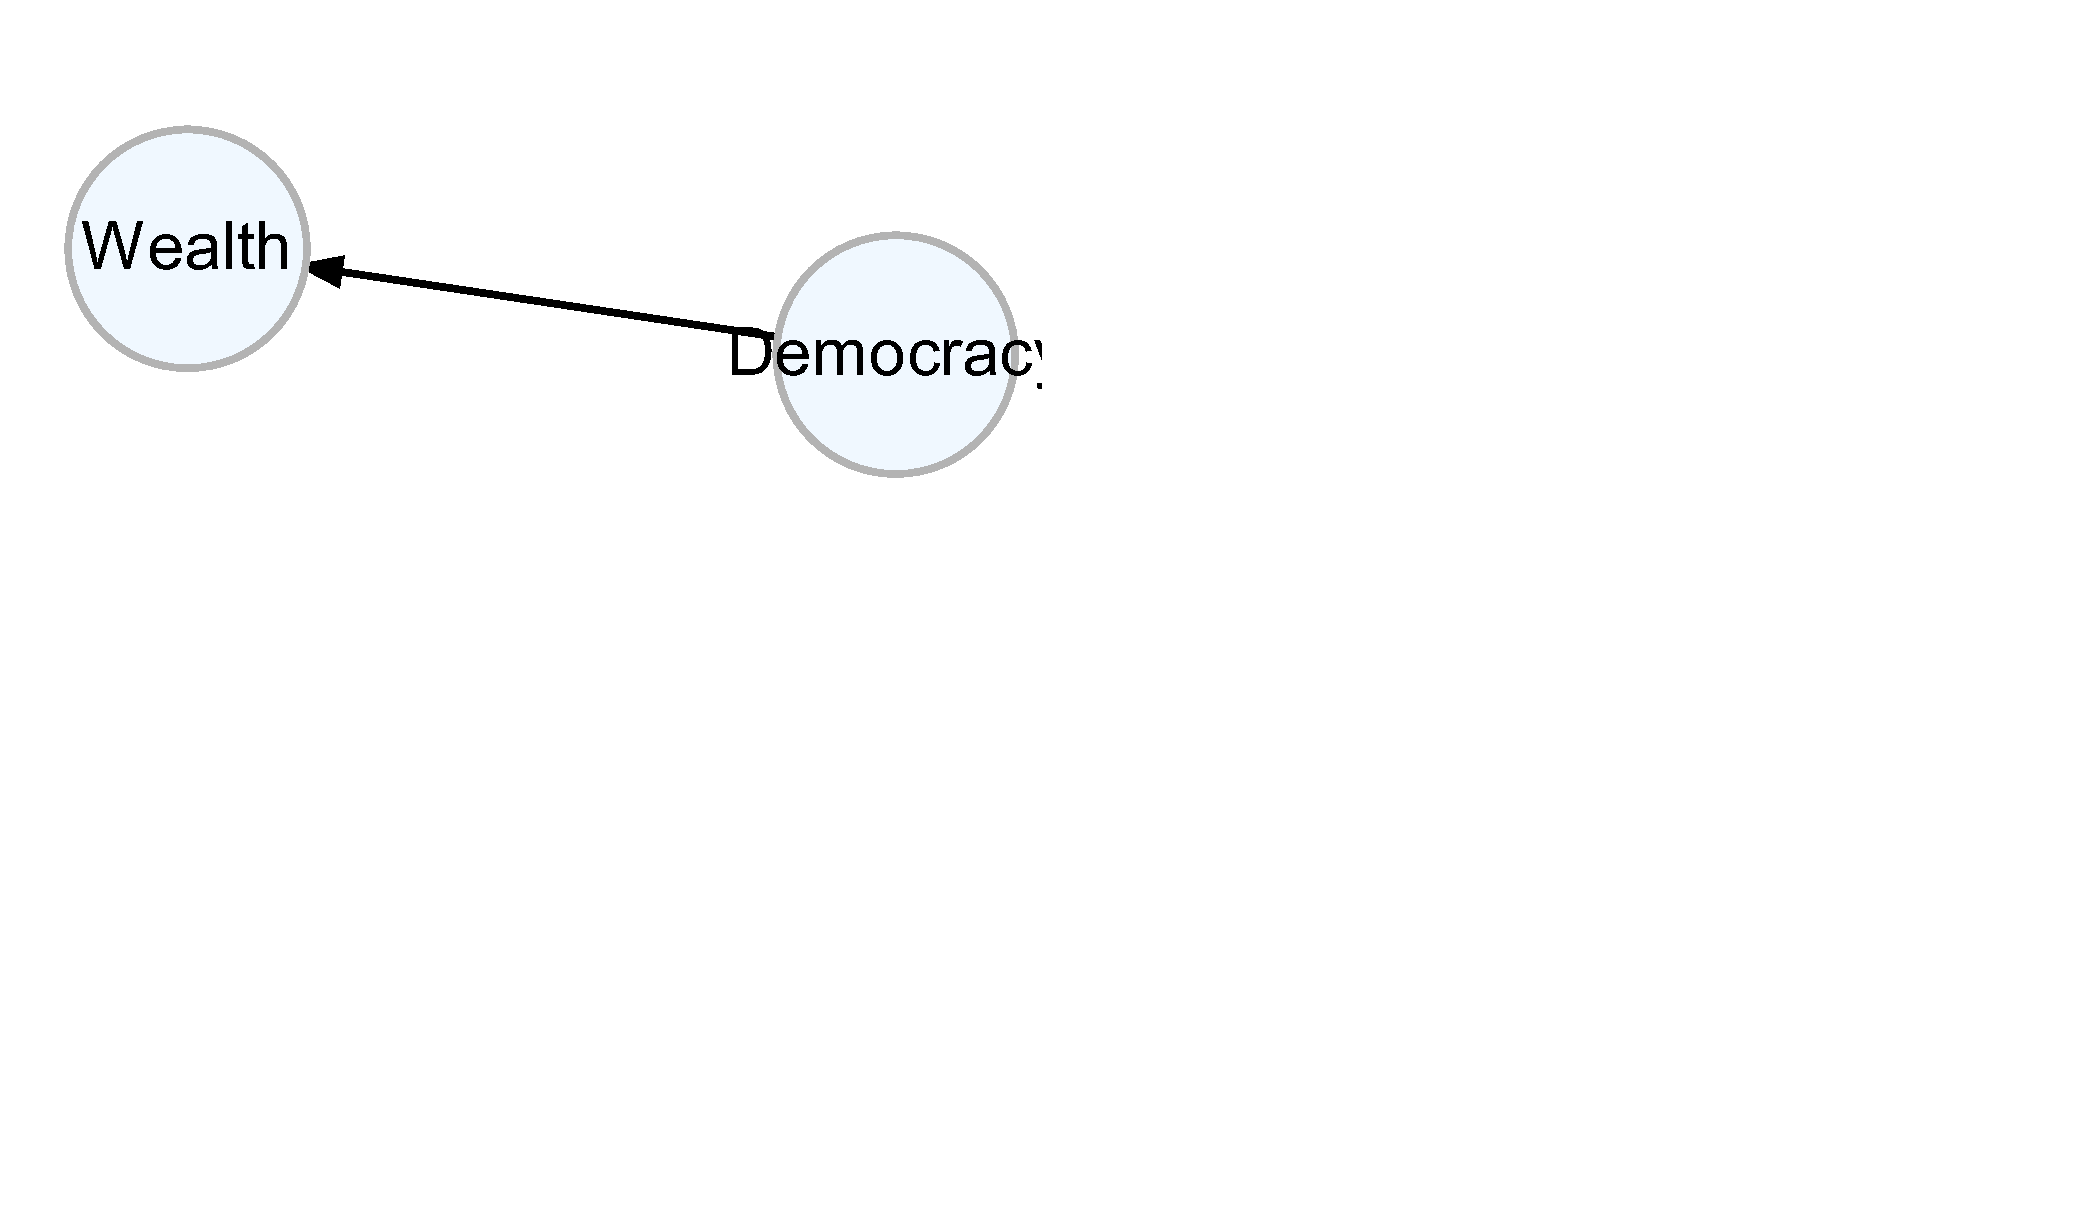
\includegraphics[width=\maxwidth]{figure/unnamed-chunk-7-1} 

\end{knitrout}
\end{frame}


\begin{frame}
\frametitle{Self-Selection Bias}
\begin{itemize}
\item Imagine a treatment assignment mechanism where people get to \textit{choose} their treatment
\end{itemize}
\begin{table}[htbp]
  \centering
  \caption{Treatment Assignment by Self-Selection}
    \begin{tabular}{|l|r|l|r|r|l|}
    \hline
          & \multicolumn{1}{l|}{D} & $Y_1$  & \multicolumn{1}{l|}{$Y_0$} & \multicolumn{1}{l|}{$Y_i$} & Real Effect \bigstrut\\
    \hline
    A     & 1     & \multicolumn{1}{r|}{\cellcolor{teal}7} & \multicolumn{1}{l|}{4} & 7     & 3 \bigstrut\\
    \hline
    B     & 1     & \multicolumn{1}{r|}{\cellcolor{teal}9} & \multicolumn{1}{l|}{5} & 9     & 4 \bigstrut\\
    \hline
    C     & 0     & 4     & \cellcolor{teal}4     & 4     & 0 \bigstrut\\
    \hline
    D     & 0     & 4     & \cellcolor{teal}3     & 3     & 1 \bigstrut\\
    \hline \pause
    $E(Y_1)=$ & & 8 & & \bigstrut\\
    \hline
    $E(Y_0)=$ & &  & 3.5 & \bigstrut\\
    \hline
    \end{tabular}%
\end{table}%
\begin{itemize}
\pause
\item ATE = 8 - 3.5 = 4.5
\item This is \textbf{self-selection bias} - treatment is affected by potential outcomes
\end{itemize}
\end{frame}

\begin{frame}
\frametitle{Problems with Observational Data}
\begin{itemize}
\item Depending on the treatment assignment mechanism we get a range of Average Treatment Effects:
\end{itemize}
\begin{table}[htbp]
  \centering
  \caption{Comparing Average Treatment Effects}
    \begin{tabular}{|l|r|}
    \hline
    \textbf{Treated Units} & \multicolumn{1}{l|}{\textbf{ATE}} \bigstrut\\
    \hline
    Real Effect for all units & 2 \bigstrut\\
    \hline
    A \& D & 1 \bigstrut\\
    \hline
    Women & -0.5 \bigstrut\\
    \hline
    Self-selection & 4.5 \bigstrut\\
    \hline
    \end{tabular}%
\end{table}%
\end{frame}

\begin{frame}
\frametitle{Problems with Observational Data}
\begin{itemize}
\item We can identify the source of these biases in potential outcomes:
\pause
\end{itemize}
\begin{multline}
\underbrace{E(Y_i|D=1)-E(Y_i|D=0)}_\text{Observed Effect}
\end{multline}
\end{frame}

\begin{frame}
\frametitle{Problems with Observational Data}
\begin{itemize}
\item We can identify the source of these biases in potential outcomes:
\end{itemize}
\begin{multline}
\underbrace{E(Y_i|D=1)-E(Y_i|D=0)}_\text{Observed Effect} = \underbrace{E(Y_{1i} - Y_{0i})}_\text{Real ATE} \\ + \underbrace{\frac{1}{2}\Big[ E(Y_{1i}|D=1) - E(Y_{1i}|D=0) \Big]}_\text{Imbalance on $Y_1$} + \underbrace{\frac{1}{2}\Big[ E(Y_{0i}|D=1) - E(Y_{0i}|D=0) \Big]}_\text{Imbalance on $Y_0$}
\end{multline}
\footnotesize
NB: For equal-sized treatment and control groups
\normalsize
\end{frame}

\begin{frame}
\frametitle{Problems with Observational Data}
\begin{itemize}
\item Disaggregating the Self-Selection Bias:
\end{itemize}
\begin{center}
\begin{multline}
\frac{(7+9-4-3)}{2} = \frac{(7+9+4+4-4-5-4-3)}{4} \\+ \frac{1}{2}\Big[ \frac{(7+9)}{2} - \frac{(4+4)}{2} \Big] + \frac{1}{2} \Big[ \frac{(4+5)}{2}- \frac{(4+3)}{2}\Big] \\
4.5 = \color{red}2 \color{black}+ 2 + \frac{1}{2}
\end{multline}
\end{center}
\end{frame}





\end{document}
 
 % effects of causes vs. reverse
